% This file contains both the handout and the text of the paper. The latter is marked by a \begin{paper}…\end{paper}; the former is unmarked but in special places where \begin{handout}…\end{handout} is explicitly written.

%%% TODO: search for יפה, מעניין/ת in the seminar paper

\documentclass[a5paper, twoside]{article}
\usepackage[top=2.0cm,bottom=2.0cm,left=2.0cm,right=2.0cm]{geometry}

\usepackage{microtype}
\usepackage{setspace, multirow, xltxtra, longtable, ltxtable, amsmath, fancybox, marginnote, rotating, needspace, enumerate, multicol, environ, paralist, tabu, paracol, parallel}

\renewcommand{\textsc}[1]{{\fontspec{TeX Gyre Pagella}\scshape#1}}
\newcommand{\textscbf}[1]{\textsc{\textbf{#1}}}

\usepackage{comment, framed}
%\specialcomment{paper}{\begin{leftbar}}{\end{leftbar}}
\excludecomment{paper}
\specialcomment{extra}{\fontsize{8}{8}\fontspec{Gentium Basic}}{\fontsize{10}{10}\fontspec{Gentium Basic}}

%\hyphenpenalty=5000
%%\tolerance=99999
%%\widowpenalty=1000
%%\clubpenalty=1000

\setlength\parskip{\medskipamount}
\setlength\parindent{0pt}

\usepackage[hidelinks]{hyperref}
%\IfFileExists{url.sty}{\usepackage{url}}
%{\newcommand{\url}{\texttt}}

\newcommand{\zero}{{\fontspec{Apple Symbols}∅}}

\newcommand{\nosic}{}

%\newcommand{\C}[1]{{\fontsize{11}{11}\fontspec[Language=Welsh]{Junicode}{#1}}}
%\newcommand{\C}[1]{{\fontspec[Language=Welsh,SmallCapsFont={LMRoman10 Caps}, HyphenChar=None]{Optima}{#1}}}
%\newcommand{\C}[1]{{\fontspec[Language=Welsh,SmallCapsFont={LMRoman10 Caps}, HyphenChar=None]{Gentium Basic}\textit{#1}}}
\newcommand{\slot}[1]{{{\textsc{#1}}}}
\newcommand{\trans}[1]{{\LR{\fontspec{TeX Gyre Pagella}\textit{#1}}}}

\usepackage[nooverlap, latin]{ruby}
\renewcommand{\rubysize}{0.75}
%\renewcommand{\rubysep}{-1cm}
%\renewcommand{\rubysep}{-0.9cm}
%\renewcommand{\ruby}[2]{#1}

%\newcommand{\gl}[2]{\ruby{#1}{\fontspec{Gill Sans Light}\mdseries\upshape #2\,}}
\newcommand{\gl}[2]{#1}
\newcommand{\Hebrew}[1]{{\RL{\fontspec[Script=Hebrew]{Guttman Hodes}#1}}}
\newcommand{\gram}[1]{{\fontspec{TeX Gyre Pagella}\textsc{#1}}}

%\newcommand{\appmargin}[1]{\marginpar{\vskip-0.5em\R{\begin{flushright}
%
%	{\scriptsize #1}\end{flushright}}}}
\newcommand{\appmargin}[1]{}

\newcommand{\Chl}[1]{\highlight{#1}}
\newcommand{\BHhl}[1]{\BHhighlight{#1}}
\newcommand{\highlight}[1]{{{\underline{#1}}}}
\newcommand{\BHhighlight}[1]{{{\underline{#1}}}}
\newcommand{\hl}[1]{\textbf{#1}}
%\newcommand{\quo}[1]{{\fontsize{8}{8}\textit{#1}}}
\newcommand{\quo}[1]{{\textit{#1}}}
\newcommand{\secu}[1]{\textbf{#1}}
%\renewcommand{\emph}[1]{\textbf{#1}}
\newcommand{\kjvit}[1]{\emph{#1}}
\newcommand{\typo}[1]{\superscript{(#1)}}

%\newcommand{\patternlimit}{{\fontspec{Apple Symbols}◇}}
\newcommand{\patternlimit}{{\fontspec{Apple Symbols}}}
\newcommand{\pattern}[1]{\patternlimit~{#1}~\patternlimit}



%%% Paper-specific %%%

\newcommand{\secref}[1]{\mbox{\LR{{\fontspec{SBL Hebrew}§}\LR{\ref{#1}}}}}
\newcommand{\sic}{\ {(\textit{sic})}}
\newcommand{\bcite}[3]{\llyfr{#1}~#2:#3}
\newcommand{\verseno}[1]{\superscript{#1}}

\newenvironment{changemargin}[2]{%
 \begin{list}{}{%
  \setlength{\topsep}{0pt}%
  \setlength{\leftmargin}{#1}%
  \setlength{\rightmargin}{#2}%
  \setlength{\listparindent}{\parindent}%
  \setlength{\itemindent}{\parindent}%
  \setlength{\parsep}{\parskip}%
 }%
\item[]}{\end{list}}

\makeatletter
\renewcommand{\section}{\@startsection{section}{1}{0mm}
	{3ex plus1ex minus1ex}%
	{\smallskipamount}{\fontspec{Gentium}\Large}}%
\renewcommand{\subsection}{\@startsection{subsection}{1}{0mm}
	{3ex plus1ex minus1ex}%
	{\smallskipamount}{\fontspec{Gentium}\large}}%
\renewcommand{\subsubsection}{\@startsection{subsubsection}{1}{0mm}
	{3ex plus1ex minus1ex}%
	{\smallskipamount}{\fontspec{Gentium}}}%
\makeatother

\usepackage{tikz}
\usetikzlibrary{arrows, decorations.pathmorphing, backgrounds, positioning, fit, petri}

\newcommand{\paradigma}[1]{\begin{tabular}{|c|}#1\end{tabular}}

\newcommand{\YHWH}{{\fontspec[HyphenChar=None]{Gentium}\textsc{{yhwh}}}}
\newcommand{\LORD}{{\textsc{\mbox{lord}}}}
\newcommand{\click}{{\fontspec{FreeSerif}✴}}
\newcommand{\point}[1]{[\textit{#1}]}
\newcommand{\optout}[1]{{\small [{#1}]}}

\newcommand{\typeA}{\textsc{type~a}}
\newcommand{\typeB}{\textsc{type~b}}
\newcommand{\typeC}{\textsc{type~c}}
\newcommand{\typeAsec}{ {\small\darkfaded(\typeA)}}
\newcommand{\typeBsec}{ {\small\darkfaded(\typeB)}}
\newcommand{\typeCsec}{ {\small\darkfaded(\typeC)}}

\usepackage[style=authoryear, backend=biber, eventdate=comp]{biblatex}
\bibliography{/home/me/library/bibliography/bibliography}
\renewcommand{\mkbibnamelast}[1]{\textsc{#1}}
\renewcommand{\subtitlepunct}{:\ }
\makeatletter
\newrobustcmd*{\parentexttrack}[1]{%
	\begingroup
	\blx@blxinit
	\blx@setsfcodes
	\blx@bibopenparen#1\blx@bibcloseparen
\endgroup}
\AtEveryCite{%
	\let\parentext=\parentexttrack%
	\let\bibopenparen=\bibopenparen%
\let\bibcloseparen=\bibcloseparen}
\renewbibmacro*{cite}{%
	\iffieldundef{shorthand}
	{\ifthenelse{\ifnameundef{labelname}\OR\iffieldundef{labelyear}}
		{\usebibmacro{cite:label}%
		\setunit{\addspace}}
		{\printnames{labelname}%
		\setunit{\nameyeardelim}}%
		% \usebibmacro{cite:labelyear+extrayear}}% DELETED
	\printtext[parens]{\usebibmacro{cite:labelyear+extrayear}}}% ADDED
{\usebibmacro{cite:shorthand}}}
\makeatother

\usepackage{graphics}

\usepackage{tikz}
\usetikzlibrary{arrows, decorations.pathmorphing, backgrounds, positioning, fit, petri}

\usepackage[normalem]{ulem}
\setlength{\fboxsep}{0.5ex}
\setlength\fboxrule{0.25ex}
\newcommand{\lhl}[1]{\fbox{#1}}
%\def\reduline{\bgroup \markoverwith{\lower3.5\p@\hbox{\footnotesize{}.}}\ULon}
\newcommand{\mydotuline}{\bgroup \markoverwith{\lower 1.0ex\hbox{.}}\ULon}
\newcommand{\hlA}[1]{\underline{\textbf{#1}}}
\newcommand{\hlB}[1]{\mydotuline{#1}}
\newcommand{\hlC}[1]{\dashuline{#1}}

\newcounter{exampleno}
\setcounter{exampleno}{0}
\newcommand{\ex}{\stepcounter{exampleno}\textbf{Ex.~\arabic{exampleno}}: }
\newcommand{\excont}{\textbf{Ex.~\arabic{exampleno}}: }
\newcommand{\exast}{\stepcounter{exampleno}\arabic{exampleno}}
\newcommand{\exgoback}{\addtocounter{exampleno}{-1}}
\newcommand{\exphantom}{\stepcounter{exampleno}}

\renewenvironment{example}[5] % #1=book, #2=chapter, #3=verse, #4=copy (of the same verse; different copies have different hightlighting), #5=shift (of verse number)
	{
	\framesubtitle{\llyfr{#1} #2:#3\ifthenelse{\not\equal{#5}{}}{*}{}}
	}
	{
	}

\newcommand{\transline}[2]{
%	\begin{savenotes}
%		\colchunk{\C{#1}}
%		\colchunk{#2}
%		\colplacechunks
%	\end{savenotes}
%	\vskip0.20em
{\Cpar{#1}\vspace{0.0em}} &
{{#2}\vspace{0.5em}}\\
}
\newcommand{\cotransline}[2]{\transline{\scriptsize#1}{\scriptsize#2}}

\usepackage{longtable}
\newenvironment{bilingquote}[0]%
{\begin{longtable}{p{0.46\linewidth}|p{0.46\linewidth}}}%
{\end{longtable}}


\newcommand{\quoling}[4]% Cymraeg, Hebrew (Latin transcription), KJV, Hebrew (Tiberean)
{
	\begin{tabular}{p{0.46\linewidth}!{\color{gray}\vrule}p{0.46\linewidth}}
		{#2} &
		{\fontspec[AutoFakeBold=3]{Gentium}#3}\\\\
		{{\small #4}} &
		{\begin{RTL}{\BH{\small#1}}\end{RTL}}
	\end{tabular}
}

\newcounter{pointno}
\setcounter{pointno}{0}
\newcommand{\hopoint}{\stepcounter{pointno}\ovalbox{\Alph{pointno}}\quad}

\usepackage{titlesec}

\usepackage{fontspec, bidi}
\setmainfont{Vesper Pro}
\setmonofont{PragmataPro}

\newcommand{\symbolglyph}[1]{{\fontspec{Symbola}#1}}
\newcommand{\symbolglyphalt}[1]{{\fontspec{DejaVu Serif}#1}}

\newcommand{\BH}[1]{\RL{\fontspec[Script=Hebrew, AutoFakeBold=3]{SBL Hebrew}#1}}
\newcommand{\bh}[1]{{\fontspec[AutoFakeBold=3]{Gentium Italic}#1}}

\newcommand{\C}[1]{{\fontspec{Vesper Pro}\textit{#1}}}
\newcommand{\Cpar}[1]{{\fontspec[Language=Welsh,SmallCapsFont={LMRoman10 Caps}, HyphenChar=None]{Gentium Basic}#1}}
\newcommand{\BHtr}[1]{{\fontspec[HyphenChar=None]{Gentium}\textit{#1}}}

\usepackage{newunicodechar}
\newunicodechar{ſ}{s}
\newunicodechar{ꝛ}{r}
\newunicodechar{·}{·\-}

\newcommand{\sectionornament}{\hspace{0.5em}{\symbolglyph{\color{faded} ⁘}}\hspace{0.5em}}

\newcommand{\sectionfont}{\normalfont}

\titleformat{\section}{\sectionfont\bfseries\Large\color{darkfaded}}{\textbf{\thesection}\sectionornament}{0.0cm}{}[\titleline{\color{faded}\titlerule}\vskip2pt\titleline{\color{faded}\titlerule}]
\titleformat{\subsection}{\sectionfont\bfseries\large\color{darkfaded}}{\textbf{\thesubsection}\sectionornament}{0.0cm}{}[{\titleline{\color{faded}\titlerule}}]
\titleformat{\subsubsection}{\sectionfont\bfseries\normalsize\color{darkfaded}}{\textbf{\thesubsubsection}\sectionornament}{0.0cm}{}[\titleline{\color{faded}\titlerule}]
\titleformat{\subsubsection}{\sectionfont\bfseries\normalsize\color{darkfaded}}{\textbf{\thesubsubsection}\sectionornament}{0.0cm}{}[\titleline{\color{faded}\titlerule}]
\titleformat{\paragraph}{\needspace{4\baselineskip}\sectionfont\bfseries\small\color{darkfaded}}{\textbf{\theparagraph}\sectionornament}{0.0cm}{}[\titleline{\color{faded}\titlerule}]
\titleformat{\subparagraph}{\needspace{4\baselineskip}\sectionfont\bfseries\small\color{darkfaded}}{\textbf{\thesubparagraph}\sectionornament}{0.0cm}{}[\titleline{\color{faded}\titlerule}]

\newcommand{\subsubsectiontext}[2]{\subsubsection[#1]{#1\hfill\faded (#2)}}
\newcommand{\paragraphtext}[2]{\paragraph[#1]{#1\hfill\faded (#2)}}
\newcommand{\subparagraphtext}[2]{\subparagraph[#1]{#1\hfill\faded (#2)}}

\newcommand{\subsubsectionoccurances}[2]{\subsubsectiontext{#1}{#2 occurances}}
\newcommand{\paragraphoccurances}[2]{\paragraphtext{#1}{#2 occurances}}
\newcommand{\subparagraphoccurances}[2]{\subparagraphtext{#1}{#2 occurances}}



\newcommand{\tounfold}[1]{{\addfontfeature{Color=0000FFFF}\symbolglyph{\addfontfeature{Color=0000FFFF}⛭}~\BH{#1}~\symbolglyph{\addfontfeature{Color=0000FFFF}⛭}}}


\begin{document}

\setstretch{1.00}

\title{\vspace{-1cm}
	\setstretch{0.75}
	{
		\Large
		\emph{llygaid [ſydd] ganddynt, ac ni welant}:\\
		Mediating Senses through Translation Choices
	}
}
\author{%
	\normalsize Júda Ronén\\[-0.1em]
	\small The Hebrew University of Jerusalem\\[-0.1em]
	\small Department of Linguistics
}
\date{
	\setstretch{1.25}
	\normalsize 15mh Còmhdhail Eadar-Nàiseanta na Ceiltis\\
	\normalsize Glaschu 2015
}
\maketitle
\thispagestyle{empty}


\vspace{-0.5cm}
{\small
\noindent
In 1588 William Morgan published his monumental Welsh translation of the Bible. This work is notable, among other aspects, in that it has the Old Testament translated directly from the original Hebrew. This fact invites comparative study of the Welsh and Hebrew texts, which may shed light on the Welsh text and language, the translation process, and (the translator’s reading of) the original text.

In this paper I will attempt a close examination of the lexical means by which Morgan translated Hebrew phrases concerning the senses (chiefly verbs of perception). The Hebrew and the Welsh lexicon and grammar are structured differently; that obliges the translator to make constant meaning-bearing choices, interpreting the text according to their reading thereof. Structural description of Morgan’s lexical choices will be at the heart of the paper.

I hope the proposed description, which is based on formal linguistic grounds and aims at understanding (Bible) translations through the lens of structural linguistic analysis, will contribute to our understanding of the 1588 Bible and its language.

(This paper broadens the scope of a paper delivered at ICCS14, in which the semantic field of ‘hearing’ was in focus. Attendance at the previous paper is not required nor assumed.)
}

~

\hrule

\vfill

\begin{center}
	\LR{\includegraphics[width=6.97cm]{ex_24-7.cy.png}}
	\hfill
	\LR{\includegraphics[width=3.6125cm]{ex_24-7.he.png}}\\
	Left: Exodus~24:7, William Morgan's Bible, 1588\\
	Right: Exodus~24:7, Leningrad Codex, 1008/9
\end{center}



\setcounter{page}{0}
\newpage

\def\contentsname{Structure}
\renewcommand{\contentspage}{} %%% uncomment if a ‘pageless’ TOC is wanted
{\setstretch{0.1}
\setlength\parskip{\smallskipamount}

\titlecontents{section} 
	[1.5cm] 
	{}
	{\LR{\contentslabel{1cm}}} 
	{}
	{\hfill\contentspage}
\titlecontents{subsection} 
	[2.5cm] 
	{}
	{\LR{\contentslabel{1cm}}} 
	{} 
	{\hfill\contentspage}
\titlecontents{subsubsection} 
	[3.5cm] 
	{}
	{\LR{\contentslabel{1cm}}} 
	{} 
	{\hfill\contentspage}

	\tableofcontents
}


\setcounter{section}{-1}
\section{Introduction}

\begin{frame}{}
	\begin{center}
		Introduction
	\end{center}
\end{frame}



\subsection{Translation as a decision process}

\begin{frame}{Bridging linguistic gap between languages}
	\includegraphics[width=0.50\textwidth]{../ps_115-5.cy.png}
	\hfill
	\includegraphics[width=0.44\textwidth]{../ps_115-5.he.png}

	\vfill

	Left: Psalms~115:5, William Morgan’s Bible, 1588\\
	Right: Psalms~115:5, Leningrad Codex, 1008/9
\end{frame}



\begin{frame}{\hopoint Translation as a decision process}
	$$
	\mtext{A} \transto
	\begin{dcases}
		\mtext{X}\\
		\mtext{Y}
	\end{dcases}
	$$

	$$
	\mtext{B} \transto
	\begin{dcases}
		\mtext{Y}
	\end{dcases}
	$$

	$$
	\mtext{C} \transto
	\begin{dcases}
		\mtext{Y}
	\end{dcases}
	$$

	$$
	\mtext{D} \transto
	\begin{dcases}
		\mtext{X}\\
		\mtext{Z}\\
		\mtext{U}\\
		\mtext{V}\\
		\mtext{W}
	\end{dcases}
	$$

	Theoretical background: \cite{levy.j:1967:translation}.
\end{frame}



\subsection{Methodology}

\begin{frame}{Methodology}
	\begin{enumerate}
		\item Making a bilingual database using a Biblical concordance (\cite{even-shoshan.a:1977:concordance})
		\item Grouping verses according to translations choices
		\item Generalisation and finding patterns
	\end{enumerate}
\end{frame}



%-%\subsection{Corpus}
%-%
%-%\begin{frame}{William Morgan’s 1588 edition}
%-%	\begin{center}
%-%		\includegraphics[width=0.9\textwidth]{images/1588.jpg}
%-%
%-%		\vfill
%-%
%-%		1588 printed Bible. Digital facsimile
%-%	\end{center}
%-%\end{frame}



\subsection{Corpus}

\begin{frame}{Corpus extent}
	\begin{itemize}
		\item \bh{rå̄ʾå̄} ‘see’ and \bh{šå̄maʿ} ‘hear’:
			\begin{itemize}
				\item {Pentateuch \quad\scriptsize (Torah, \bh{tōrå̄})}
			\end{itemize}
		\item all other words and collocations: the whole bible
			\begin{itemize}
				\item {Pentateuch \quad\scriptsize (Torah, \bh{tōrå̄})}
				\item {Prophets \quad\scriptsize (Nevi’im, \bh{nəḇīʾīm})}
				\item {Writings \quad\scriptsize (Ketuvim, \bh{kəṯūḇīm})}
			\end{itemize}
	\end{itemize}
\end{frame}



\subsection{ICCS14}

\begin{frame}{ICCS14}
	\begin{center}
		\includegraphics[width=0.9\textwidth]{images/ICCS14.pdf}
	\end{center}
\end{frame}


\tounfold{גניבת ברכת יצחק (1:27:1,(5),12,21,22)}


\section{Senses}

\sepslide{The Senses}

\subsection{Overiew}

\begin{paper}
	{\click} The first question one has to ask oneself when approaching our topic is ‘\hl{what are the senses in question?}’. To try and answer this question with respect to the Bible we will have to deviate to antropology, theology, literary theory, cognitive science and other fields. Unfortunately, we don’t have to do this…

	In a recent publication, \cite{avrahami.y:2012:senses} came to the conclusion of a \hl{septasensory} model for biblical epistemology: sight, hearing, kinaesthesia, speech, taste/eating, smell and touch. This model is not uncontroversial, {\click} and for our current purposes we will use the (Western) \hl{pentasensory} model, which is more familiar to us.
\end{paper}

\begin{hopoint}
	\begin{tabular}{ll@{\quad→\quad}l}
		\textbf{sight}   & \bh{råʾå}   & \C{gweled, edrych, …}\\
		\textbf{hearing} & \bh{šåmaʿ}  & \C{clywed, gwrando, …}\\
		\textbf{touch}   & \bh{måšaš}  & \C{teimlo, …}\\
		\textbf{smell}   & \bh{hērīaḥ} & \C{arogli, …}\\
		\textbf{taste}   & \bh{ṭåʿam}  & \C{archwaithu, …}
	\end{tabular}
\end{hopoint}

\begin{paper}
\point{point} These are the most common \hl{Hebrew verbs} for these modalities and their most common \hl{translations}.

\tounfold{לפרט על השלושנקודות ומה אני עושה כאן}
\end{paper}



\subsubsection{Lists of modalities}

\tounfold{לכלול את:
	דניאל 5:23
	שאר הדוגמאות שמצאתי בעבודה הסמינריונית
	החלק הרלוונטי ב„חושים” במסד הנתונים}

\begin{example}{5}{4}{28}{}{}
	\quoling
	{וַעֲבַדְתֶּם־שָׁ֣ם אֱלֹהִ֔ים מַעֲשֵׂ֖ה יְדֵ֣י אָדָ֑ם עֵ֣ץ וָאֶ֔בֶן אֲשֶׁ֤ר לֹֽא־\hlA{יִרְאוּן֙} וְלֹ֣א \hlA{יִשְׁמְע֔וּן} וְלֹ֥א \hlA{יֹֽאכְל֖וּן} וְלֹ֥א \hlA{יְרִיחֻֽן}׃}
	{Ac yno y gwaſanaethwch dduwiau [o] waith dwylo dŷn, [ſef] pꝛen, a maen, y rhai ni \hlA{welant}, ac ni \hlA{chlywant}, ac ni \hlA{fwyttânt}, ac ni \hlA{aroglant}.}
	{wa·ʿăḇaḏtɛm·šåm ʾɛ̆lōhīm maʿăśē yəḏē ʾåḏåm ʿēṣ wå·ʾɛḇɛn ʾăšɛr lō·\hlA{yirʾūn} wə·lō \hlA{yišməʿūn} wə·lō \hlA{yōḵlūn} wə·lō \hlA{yərīḥun}}
	{And there ye shall serve gods, the work of men’s hands, wood and stone, which neither \hlA{see}, nor \hlA{hear}, nor \hlA{eat}, nor \hlA{smell}.}
\end{example}

\begin{example}{Ps}{115}{4–7}{}{}
	\quoling
	{%
		\textsuperscript{4}~עֲצַבֵּיהֶם כֶּ֣סֶף וְזָהָ֑ב מַ֝עֲשֵׂ֗ה יְדֵ֣י אָדָֽם׃
		\textsuperscript{5}~פֶּֽה־לָ֭הֶם וְלֹ֣א \hlA{יְדַבֵּ֑רוּ} עֵינַ֥יִם לָ֝הֶ֗ם וְלֹ֣א \hlA{יִרְאֽוּ}׃
		\textsuperscript{6}~אָזְנַ֣יִם לָ֭הֶם וְלֹ֣א \hlA{יִשְׁמָ֑עוּ} אַ֥ף לָ֝הֶ֗ם וְלֹ֣א \hlA{יְרִיחֽוּן}׃
		\textsuperscript{7}~יְדֵיהֶ֤ם ׀ וְלֹ֬א \hlA{יְמִישׁ֗וּן} רַ֭גְלֵיהֶם וְלֹ֣א \hlA{יְהַלֵּ֑כוּ} לֹֽא־\hlA{יֶ֝הְגּ֗וּ} בִּגְרוֹנָֽם׃
	}
	{%
		\textsuperscript{4}~Eu delwau hwy [ydynt] o aur, ac arian, [ſef] o waith dynnion.
		\textsuperscript{5}~Genau [ſydd] iddynt, ac ni \hlA{lefarant}, llygaid [ſydd] ganddynt, ac ni \hlA{welant}.
		\textsuperscript{6}~[Y mae] cluſtiau iddynt, ac ni \hlA{chlywant}, ffroenau [ſydd] ganddynt, ac ni \hlA{aroglant}.
		\textsuperscript{7}~Dwylo [ſydd] iddynt, ac ni \hlA{theimlant}: traed [ſy] iddynt, ac ni \hlA{cherddant}: ni \hlA{leiſiant} [ychwaith] ai gwddf.
	}
	{%
		\textsuperscript{4}~ʿăṣabbēhɛm kɛsɛp̄ wə·zåhåḇ maʿăśē yəḏē ʾåḏåm
		\textsuperscript{5}~pɛ·l·åhɛm wə·lō \hlA{yəḏabbērū} ʿēnayim l·åhɛm wə·lō \hlA{yirʾū}
		\textsuperscript{6}~ʾåznayim l·åhɛm wə·lō \hlA{yišmåʿū} ʾap̄ l·åhɛm wə·lō \hlA{yərīḥūn}
		\textsuperscript{7}~yəḏēhɛm wə·lō \hlA{yəmīšūn} raḡlēhɛm wə·lō \hlA{yəhallēḵū }lō·\hlA{yɛhgū} bi·ḡrōnåm
	}
	{%
		\textsuperscript{4}~Their idols \textit{are} silver and gold, the work of men’s hands.
		\textsuperscript{5}~They have mouths, but they \hlA{speak} not: eyes have they, but they \hlA{see} not:
		\textsuperscript{6}~They have ears, but they \hlA{hear} not: noses have they, but they \hlA{smell} not:
		\textsuperscript{7}~They have hands, but they \hlA{handle} not: feet have they, but they \hlA{walk} not: neither \hlA{speak} they through their throat.
	}
\end{example}



\subsubsection{\C{gweled}:\C{edrych} and \C{clywed}:\C{gwrando}}

\begin{paper}
	{\click} The \hl{key lexical distinctions} Morgan had to make when translating instances of the common verbs \bh{råʾå} ‘to see’ and \bh{šåmaʿ} ‘to hear’ are between \C{gweled} and \C{edrych}, and \C{clywed} and \C{gwrando}, respectively.

	{\click} The \hl{value} of these choices is, in the nutshell, that:
	\begin{compactitem}
		\item \C{gweled} and \C{clywed} designate simple, semantically unmarked \hl{sensory perception}, as well as perception of \hl{content} (seeing or hearing that something is such and such).
		\item \C{edrych} and \C{gwrando}, on the other hand, are marked with \hl{non-sensory meaning}, whether involving actual sensory perception or not.
			\begin{compactitem}
				\item For \C{edrych} this includes facing (with indication of direction or without it), looking at (\tounfold{}) with for (with \C{am}), accepting, examining etc.
				\item For \C{gwrando} this includes obeying, accepting, following, judging, interpreting, etc.
			\end{compactitem}
	\end{compactitem}

	So, as one can expect from this, in the lists of modalities we’ve talked about \C{gweled} and \C{clywed}, not \C{edrych} and \C{gwrando}, are found.
\end{paper}

%*** \begin{hopoint}
%*** 	\begin{tabular}{l|cc}
%*** 		& {sensory} & {\ruby{additional}{(non-sensory)} meaning}\\
%*** 		\hline
%*** 		\C{gweled}, \C{clywed}  & + & -\\
%*** 		\C{edrych}, \C{gwrando} & ± & +
%*** 	\end{tabular}
%*** \end{hopoint}

\tounfold{דוגמה להכניס איפשהו:}

\begin{example}{Job}{35}{13}{}{}
	\quoling
	{אַךְ־שָׁ֭וְא לֹא־\highlight{יִשְׁמַ֥ע} ׀ אֵ֑ל וְ֝שַׁדַּ֗י לֹ֣א \highlight{יְשׁוּרֶֽנָּה}׃}
	{Diau na \highlight{wꝛendu} Duw oferedd: ac nad \highlight{edꝛych} yꝛ Holl-alluoc arno.}
	{ʾaḵ·šåw lō·\highlight{yišmaʿ} ʾēl wə·šadday lō \highlight{yəšūrɛnnå}}
	{Surely God will not \highlight{hear} vanity, neither will the Almighty \highlight{regard} it.}
\end{example}

\tounfold{***יכולת כללית תמיד הפשוט; פעולה מורכבת מסויימת תמיד המורכב}


\subsection{Sight}

\sepslide{Sight}



\subsubsection{\bh{rå̄ʾå̄}}

\begin{frame}{\bh{rå̄ʾå̄} ‘to see’}
	\begin{center}
		$$
		\mtext{\bh{rå̄ʾå̄}} \transto
		\begin{dcases}
			\C{\hl{gweled}}\\
			\C{\hl{edrych}}\\
			\mtext{\small\C{(canfod)}}
		\end{dcases}
		$$

		$$
		\mtext{\bh{hɛrʾå̄} \gram{(caus.)}} \transto
		\begin{dcases}
			\C{\hl{dangos}}\\
			\mtext{\small\C{(peri + gweled)}}
		\end{dcases}
		$$

		$$
		\mtext{\bh{nirʾå̄} \gram{(pass.)}} \transto
		\begin{dcases}
			\C{\hl{ymddangos}}\\
			\mtext{\small\C{(gweled \gram{(pass.))}}}
		\end{dcases}
		$$
	\end{center}
\end{frame}


\begin{frame}{\ex Sensory perception}
	\begin{example}{Ex.}{10}{23}{}{}
		\quoling
		{לֹֽא־\lhl{רָא֞וּ} אִ֣ישׁ אֶת־אָחִ֗יו וְלֹא־קָ֛מוּ אִ֥ישׁ מִתַּחְתָּ֖יו שְׁלֹ֣שֶׁת יָמִ֑ים וּֽלְכָל־בְּנֵ֧י יִשְׂרָאֵ֛ל הָ֥יָה א֖וֹר בְּמוֹשְׁבֹתָֽם׃}
		{Ni \lhl{wele} neb ei gilydd, ac ni chododd neb oi le dꝛi diwꝛnod: ond yꝛ ydoedd goleuni i holl feibion Iſrael yn eu trigfannau.}
		{lō·\lhl{rå̄ʾū} ʾīš ʾɛṯ·ʾå̄ḥīw wə·lō·qå̄mū ʾīš mit·taḥtå̄w šəlōšɛṯ yå̄mīm ū·l·ḵå̄l·bənē yiśrå̄ʾēl hå̄yå̄ ʾōr bə·mōšḇōṯå̄m}
		{They \lhl{saw} not one another, neither rose any from his place for three days: but all the children of Israel had light in their dwellings.}
	\end{example}
\end{frame}


\begin{frame}{\ex Sensory perception}
	\begin{example}{Num.}{13}{33}{}{}
		\quoling
		{וְשָׁ֣ם \lhl{רָאִ֗ינוּ} אֶת־הַנְּפִילִ֛ים בְּנֵ֥י עֲנָ֖ק מִן־הַנְּפִלִ֑ים וַנְּהִ֤י בְעֵינֵ֙ינוּ֙ כַּֽחֲגָבִ֔ים וְכֵ֥ן הָיִ֖ינוּ בְּעֵינֵיהֶֽם׃}
		{Ac yno y \lhl{gwelſom} feibion Anac y cawꝛi [y rhai a ddaethant] o’ꝛ cawꝛi, ac yꝛ oeddem yn ein golwg ein hunain fel ceiliogod rhedyn, ac felly yꝛ oeddem yn eu golwg hwyntau.}
		{wə·šå̄m \lhl{rå̄ʾīnū} ʾɛṯ·han·nəp̄īlīm bənē ʿănå̄q min·han·nəp̄īlīm wan·nəhī ḇə·ʿēnēnū ka·ḥăḡå̄ḇīm wə·ḵēn hå̄yīnū bə·ʿēnēhɛm}
		{And there we \lhl{saw} the giants, the sons of Anak, \emph{which come} of the giants: and we were in our own sight as grasshoppers, and so we were in their sight.}
	\end{example}
\end{frame}


\begin{frame}{\ex Content (\bh{kī} ‘that’)}
	\begin{example}{Gen.}{1}{4}{}{}
		\quoling
		{\lhl{וַיַּ֧רְא} אֱלֹהִ֛ים אֶת־הָא֖וֹר \hlA{כִּי}־ט֑וֹב וַיַּבְדֵּ֣ל אֱלֹהִ֔ים בֵּ֥ין הָא֖וֹר וּבֵ֥ין הַחֹֽשֶׁךְ׃}
		{Yna Duw a \lhl{welodd} y goleuni \hlA{mai} dâ [oedd,] a Duw a wahanodd rhwng y goleuni a’r tywyllwch.}
		{way·\lhl{yar} ʾɛ̆lōhīm ʾɛṯ·hå̄·ʾōr \hlA{kī}·ṭōḇ way·yaḇdēl ʾɛ̆lōhīm bēn hå̄·ʾōr ū·ḇēn ha·ḥōšɛḵ}
		{And God saw the light, \hlA{that} \emph{it was} good: and God divided the light from the darkness.}
	\end{example}
\end{frame}


\begin{frame}{\ex Content (\bh{kī} ‘that’)}
	\begin{example}{Gen.}{37}{4}{}{}
		\quoling
		{\lhl{וַיִּרְא֣וּ} אֶחָ֗יו \hlA{כִּֽי}־אֹת֞וֹ אָהַ֤ב אֲבִיהֶם֙ מִכָּל־אֶחָ֔יו וַֽיִּשְׂנְא֖וּ אֹת֑וֹ וְלֹ֥א יָכְל֖וּ דַּבְּר֥וֹ לְשָׁלֹֽם׃}
		{Pan \lhl{welodd} ei frodyꝛ, \hlA{fod} eu tâd \hlA{yn} ei garu ef yn fwy nai holl frodyꝛ: yna hwy ai caſaſant ef, ac ni fedꝛent ymddiddan [ag] ef yn heddychol.}
		{way·\lhl{yirʾū} ʾɛḥå̄w \hlA{kī}·ʾōṯ·ō ʾå̄haḇ ʾăḇīhɛm mik·kå̄l·ʾɛḥå̄w way·yiśnəʾū ʾōṯ·ō wə·lō yå̄ḵlū dabbərō lə·šå̄lōm}
		{And when his brethren \lhl{saw} \hlA{that} their father loved him more than all his brethren, they hated him, and could not speak peaceably unto him.}
	\end{example}
\end{frame}


\begin{frame}{\ex Inspection}
	\begin{example}{Num.}{13}{18}{}{}
		\quoling
		{\lhl{וּרְאִיתֶ֥ם} אֶת־הָאָ֖רֶץ מַה־הִ֑וא וְאֶת־הָעָם֙ הַיֹּשֵׁ֣ב עָלֶ֔יהָ הֶחָזָ֥ק הוּא֙ הֲרָפֶ֔ה הַמְעַ֥ט ה֖וּא אִם־רָֽב׃}
		{Ac \lhl{edꝛychwch} y wlad beth yw hi, a’r bobl ſydd yn trigo ynddi, ai cryf, ai gwan, ai llawer [ydynt.]}
		{ū·\lhl{rʾīṯɛm} ʾɛṯ·hå̄·ʾå̄rɛṣ ma·hī wə·ʾɛṯ·hå̄·ʿå̄m hay·yōšēḇ ʿå̄lɛhå̄ hɛ·ḥå̄zå̄q hū hă·rå̄p̄ɛ ha·mʿaṭ hū ʾim·rå̄ḇ}
		{And \lhl{see} the land, what it \kjvit{is}; and the people that dwelleth therein, whether they \kjvit{be} strong or weak, few or many;}
	\end{example}
\end{frame}


\begin{frame}{\ex Inspection}
	\begin{example}{Num.}{32}{8}{}{}
		\quoling
		{כֹּ֥ה עָשׂ֖וּ אֲבֹתֵיכֶ֑ם בְּשָׁלְחִ֥י אֹתָ֛ם מִקָּדֵ֥שׁ בַּרְנֵ֖עַ \lhl{לִרְא֥וֹת} אֶת־הָאָֽרֶץ׃}
		{Felly y gwnaeth eich tadau, pan anfonais hwynt o Cades Barnea i \lhl{edꝛych} y tîr.}
		{kō ʿå̄śū ʾăḇōṯēḵɛm bə·šå̄lḥī ʾōṯå̄·m miq·qå̄ḏēš barnēaʿ li·\lhl{rʾōṯ} ʾɛṯ·hå̄·ʾå̄rɛṣ}
		{Thus did your fathers, when I sent them from Kadeshbarnea to \lhl{see} the land.}
	\end{example}
\end{frame}


\begin{frame}{\ex Priestly examination of leprosy}
	\begin{example}{Lev.}{13}{8}{}{}
		\quoling
		{\lhl{וְרָאָה֙} הַכֹּהֵ֔ן וְהִנֵּ֛ה פָּשְׂתָ֥ה הַמִּסְפַּ֖חַת בָּע֑וֹר וְטִמְּא֥וֹ הַכֹּהֵ֖ן צָרַ֥עַת הִֽוא׃}
		{Ac \lhl{edꝛyched} yꝛ offeiriad, ac os lledodd y grammen yn y croen, yna barned yꝛ offeiriad ef yn aflan: gwahan-glwyf yw hwnnw.}
		{wə·\lhl{rå̄ʾå̄} hak·kōhēn wə·hinnē på̄śṯå̄ ham·mispaḥaṯ b·å̄·ʿōr wə·ṭimməʾō hak·kōhēn ṣå̄raʿaṯ hī}
		{And \emph{if} the priest \lhl{see} that, behold, the scab spreadeth in the skin, then the priest shall pronounce him unclean: it \emph{is} a leprosy.}
	\end{example}
\end{frame}



\subsubsection{\bh{på̄nå̄}}

\begin{frame}{\bh{på̄nå̄} ‘to turn, to face, to look’}
	\begin{center}
		$$
		\mtext{\bh{på̄nå̄}} \transto
		\begin{dcases}
			\C{\hl{edrych}}\\
			\C{\hl{troi}}\\
			\mtext{\small\C{(dychwelyd, wynebu, …)}}
		\end{dcases}
		$$
	\end{center}
\end{frame}


\begin{frame}{\bh{på̄nå̄} being translated by \C{edrych}}
	\begin{itemize}
		\item looking\hfill\exvref{Ex.}{2}{12}{}
		\item accepting or willing {\small (with \C{ar} or \C{am})}\hfill\exvref{2 Chr.}{6}{19}{}
		\item a geographical direction {\small (with \C{tua})}\hfill\exvref{Ezek.}{43}{1}{}
	\end{itemize}
\end{frame}


\begin{frame}{\exwref \bh{på̄nå̄} → \C{edrych} (looking)}
	\exstep
	\begin{example}{Ex.}{2}{12}{}{}
		\quoling
		{\lhl{וַיִּ֤פֶן} כֹּה֙ וָכֹ֔ה וַיַּ֖רְא כִּ֣י אֵ֣ין אִ֑ישׁ וַיַּךְ֙ אֶת־הַמִּצְרִ֔י וַֽיִּטְמְנֵ֖הוּ בַּחֽוֹל׃}
		{Ac efe a \lhl{edꝛychodd} ymma, ac accw, a phan welodd nad [oedd yno] neb: yna efe a laddodd yꝛ Aiphtiad, ac ai cuddiodd yn y tyfod.}
		{way·\lhl{yīp̄ɛn} kō wå̄·ḵō way·yar kī ʾēn ʾīš way·yaḵ ʾɛṯ·ham·miṣrī wayyiṭmənēhū b·a·ḥōl}
		{And he \lhl{looked} this way and that way, and when he saw that \kjvit{there was} no man, he slew the Egyptian, and hid him in the sand.}
	\end{example}
\end{frame}


\begin{frame}{\exwref \bh{på̄nå̄} → \C{edrych} (accepting or willing)}
	\exstep
	\begin{example}{2 Chr.}{6}{19}{}{}
		\quoling
		{\lhl{וּפָנִ֜יתָ} \hlA{אֶל}־תְּפִלַּ֧ת עַבְדְּךָ֛ וְאֶל־תְּחִנָּת֖וֹ יְהוָ֣ה אֱלֹהָ֑י לִשְׁמֹ֤עַ אֶל־הָרִנָּה֙ וְאֶל־הַתְּפִלָּ֔ה אֲשֶׁ֥ר עַבְדְּךָ֖ מִתְפַּלֵּ֥ל לְפָנֶֽיךָ׃}
		{\lhl{Edꝛych} gan hynny \hlA{ar} weddi dy wâs, ac ar ei ddeiſyfiad ef ô Arglwydd fy Nuw: i wꝛando ar y llêf, ac ar y weddi yꝛ hon y mae dy wâs yn ei gweddio ger dy fron di.}
		{ū·\lhl{p̄å̄nīṯå̄} \hlA{ʾɛl}·təp̄illaṯ ʿaḇdəḵå̄ wə·ʾɛl·təḥinnå̄ṯō {\YHWH} ʾɛ̆lōhå̄y li·šmōaʿ ʾɛl·hå̄·rinnå̄ wə·ʾɛl·hat·təp̄illå̄ ʾăšɛr ʿaḇdəḵå̄ miṯpallēl lə·p̄å̄nɛḵå̄}
		{\lhl{Have respect} therefore \hlA{to} the prayer of thy servant, and to his supplication, O {\LORD} my God, to hearken unto the cry and the prayer which thy servant prayeth before thee:}
	\end{example}
\end{frame}


\begin{frame}{\exwref \bh{på̄nå̄} → \C{edrych} (geographical direction)}
	\exstep
	\begin{example}{Ezek.}{43}{1}{}{}
		\quoling
		{וַיּוֹלִכֵ֖נִי אֶל־הַשָּׁ֑עַר שַׁ֕עַר אֲשֶׁ֥ר \lhl{פֹּנֶ֖ה} דֶּ֥רֶךְ הַקָּדִֽים׃}
		{Ac efe a’m dug fi i’r poꝛth [ſef] y poꝛth yꝛ hwn ſydd yn \lhl{edꝛych} \hlA{tua} ’r dwyꝛain.}
		{wayyōlīḵēnī ʾɛl·haš·šå̄ʿar šaʿar ʾăšɛr pōnɛ dɛrɛḵ haq·qå̄ḏīm}
		{Afterward he brought me to the gate, \kjvit{even} the gate that looketh toward the east:}
	\end{example}
\end{frame}


\begin{frame}{\bh{på̄nå̄} being translated by \C{troi}}
	\begin{itemize}
		\item physical sense (+motion)\hfill\exvref{Gen.}{18}{22}{}
		\item metaphorically, turning unto other gods\hfill\exvref{Deut.}{31}{18}{}
	\end{itemize}
\end{frame}


\begin{frame}{\exwref \bh{på̄nå̄} → \C{troi} (physical sense)}
	\exstep
	\begin{example}{Gen.}{18}{22}{}{}
		\quoling
		{\lhl{וַיִּפְנ֤וּ} מִשָּׁם֙ הָֽאֲנָשִׁ֔ים וַיֵּלְכ֖וּ סְדֹ֑מָה וְאַ֨בְרָהָ֔ם עוֹדֶ֥נּוּ עֹמֵ֖ד לִפְנֵ֥י יְהוָֽה׃}
		{A [dau] oꝛ gwŷꝛ a \lhl{dꝛoeſant} oddi yno, ac a aethant tua Sodoma, ac Abꝛaham yn ſefyll \typo{fefyll} etto ger bꝛon yꝛ Arglwydd.}
		{way·\lhl{yip̄nū} miš·šå̄m hå̄·ʾănå̄šīm way·yēlḵū səḏōm·å̄ wə·ʾaḇrå̄hå̄m ʿōḏɛnnū ʿōmēḏ li·p̄nē {\YHWH}}
		{And the men \lhl{turned their faces} from thence, and went toward Sodom: but Abraham stood yet before the {\LORD}.}
	\end{example}
\end{frame}


\begin{frame}{\exwref \bh{på̄nå̄} → \C{troi} (metaphorically)}
	\exstep
	\begin{example}{Deut.}{31}{18}{}{}
		\quoling
		{וְאָנֹכִ֗י הַסְתֵּ֨ר אַסְתִּ֤יר פָּנַי֙ בַּיּ֣וֹם הַה֔וּא עַ֥ל כָּל־הָרָעָ֖ה אֲשֶׁ֣ר עָשָׂ֑ה כִּ֣י \lhl{פָנָ֔ה} אֶל־אֱלֹהִ֖ים אֲחֵרִֽים׃}
		{Canys myfi gan guddio a guddiaf fy wyneb y dydd hwnnw, am yꝛ holl ddꝛygioni ’r hyn a wnaeth efe, pan \lhl{dꝛôdd} at dduwiau dieithꝛ.}
		{wə·ʾå̄nōḵī hastēr ʾastīr på̄nay b·ay·yōm ha·hū ʿal kå̄l·hå̄·rå̄ʿå̄ ʾăšɛr ʿå̄śå̄ kī \lhl{p̄å̄nå̄} ʾɛl·ʾɛ̆lōhīm ʾăḥērīm}
		{And I will surely hide my face in that day for all the evils which they shall have wrought, in that they are \lhl{turned} unto other gods.}
	\end{example}
\end{frame}


\subsubsection{\bh{hibbīṭ}}

\subsubsection{\bh{ḥå̄zå̄}}

\begin{frame}{\bh{ḥå̄zå̄} ‘to see, to prophesy’}
	\begin{center}
		$$
		\mtext{\bh{ḥå̄zå̄}} \transto
		\begin{dcases}
			\C{\hl{gweled}}\\
			\mtext{\small\C{(…)}}
		\end{dcases}
		$$
	\end{center}
\end{frame}


\begin{frame}{\ex \bh{ḥå̄zå̄}}
	\begin{example}{Isa.}{2}{1}{}{}
		\quoling
		{הַדָּבָר֙ אֲשֶׁ֣ר \lhl{חָזָ֔ה}	יְשַֽׁעְיָ֖הוּ בֶּן־אָמ֑וֹץ עַל־יְהוּדָ֖ה וִירוּשָׁלִָֽם׃}
		{Y gair yꝛ hwn a \lhl{welodd} Eſay mab Amos am Iuda, ac Ieruſalem.}
		{had·då̄ḇå̄r ʾăšɛr \lhl{ḥå̄zå̄} yəšaʿyå̄hū bɛn·ʾå̄mōṣ ʿal·yəhūḏå̄ wī·rūšå̄lå̄yim}
		{The word that Isaiah the son of Amoz \lhl{saw} concerning Judah and Jerusalem.}
	\end{example}
\end{frame}

\begin{frame}{\ex \bh{rå̄ʾå̄} and \bh{ḥå̄zå̄}, lexical differentiation}
	\begin{example}{Isa.}{30}{10}{}{}
		\quoling
		{אֲשֶׁ֨ר אָמְר֤וּ \hlA{לָֽרֹאִים֙} לֹ֣א \hlA{תִרְא֔וּ} \lhl{וְלַ֣חֹזִ֔ים} לֹ֥א \lhl{תֶחֱזוּ}־לָ֖נוּ נְכֹח֑וֹת דַּבְּרוּ־לָ֣נוּ חֲלָק֔וֹת \lhl{חֲז֖וּ} מַהֲתַלּֽוֹת׃}
		{Y rhai a ddywedaſant wꝛth y rhai a \hlA{welant}, na \hlA{welwch}, ac wꝛth y rhai a \lhl{ganfyddant}, na \lhl{chanfyddwch} i ni gymwyſdꝛa: treuthwch i ni weniaith, \lhl{cenfyddwch} i ni ſiomedigaeth.}
		{ʾăšɛr ʾå̄mrū l·å̄·\hlA{rōʾīm} lō \hlA{ṯirʾū} wə·l·a·\lhl{ḥōzīm} lō \lhl{ṯɛḥɛ̆zū}·lå̄nū nəḵōḥōṯ dabbərū·lå̄nū ḥălå̄qōṯ \lhl{ḥăzū} mahăṯallōṯ}
		{Which say to the \hlA{seers}, \hlA{See} not; and to the \lhl{prophets}, \lhl{Prophesy} not unto us right things, speak unto us smooth things, \lhl{prophesy} deceits:}
	\end{example}
\end{frame}



\subsubsection{\bh{ṣå̄p̄å̄}}

\begin{frame}{\bh{ṣå̄p̄å̄} ‘to watch’}
	\begin{center}
		$$
		\mtext{\bh{ṣå̄p̄å̄}} \transto
		\begin{dcases}
			\mtext{\C{\hl{edrych}} (6)}\\
			\mtext{\C{disgwil} (3)}\\
			\mtext{\C{gwilio} (2)}\\
			\mtext{\C{craffu} (2)}\\
			\mtext{\C{canfod} (2)}\\
		\end{dcases}
		$$

		$$
		\mtext{\bh{ṣōp̄ɛ}} \transto
		\begin{dcases}
			\mtext{\C{\hl{gwiliedudd}} (12)}\\
			\mtext{\C{gwili-wr} (5)}\\
			\mtext{\small\C{disgwil-wr (1)}}
		\end{dcases}
		$$
	\end{center}
\end{frame}

\subsubsection{\bh{hišqīp̄}~/ \bh{nišqå̄p̄}}
\subsubsection{\bh{šå̄r}}
\subsubsection{\bh{på̄qaḥ}}
\subsubsection{\bh{šå̄zap̄}}

\subsubsection{Conclusion}

\begin{frame}{Types of translation relationships}
	\begin{itemize}
		\item Simple:
			\bh{hɛrʾå̄}, \bh{nirʾå̄}, \bh{hibbīṭ}, \bh{ḥå̄zå̄}, \bh{hišgīaḥ}, \bh{rōʾɛ}, \bh{ḥōzɛ}.
		\item Two main options:
			\bh{rå̄ʾå̄}, \bh{på̄nå̄}.
		\item More variance:
			\bh{ṣå̄p̄å̄}.
	\end{itemize}
\end{frame}


\subsection{Hearing}

\subsubsection{\bh{šåmaʿ}}

\subsubsection{\bh{hɛʾɛ̆zīn}}

\subsubsectionoccurances{\bh{hiṭṭå}~+ \bh{ʾōzɛn}}{26}

\begin{paper}
	There is an idiomatic collocation of \bh{hiṭṭå} ‘to incline’ and \bh{ʾōzɛn} ‘ear’. This collocation is translated literally mostly by \C{gogwydd} or \C{gostwng} with \C{clust} ‘ear’ as an object. These two lexemes have about the equal number of occurances, and I couldn’t find any clear-cut distinction in their use. \bh{hiṭṭå} is translated with \C{***gŵyro} once.

	Almost all occurances of \bh{hiṭṭå ʾōzɛn}, with a few exceptions from Psalms, collocate also with verbs of hearing and accepting: ‘incline your ear and hear (that is, accept)’. \bh{šåmaʿ} in this position is expectably translated by \C{gwrando}.
\end{paper}

\begin{example}{Isa.}{55}{3}{}{}
	\quoling
	{\lhl{הַטּ֤וּ} \hlA{אָזְנְכֶם֙} וּלְכ֣וּ אֵלַ֔י \hlB{שִׁמְע֖וּ} וּתְחִ֣י נַפְשְׁכֶ֑ם וְאֶכְרְתָ֤ה לָכֶם֙ בְּרִ֣ית עוֹלָ֔ם חַֽסְדֵ֥י דָוִ֖ד הַנֶּאֱמָנִֽים׃}
	{\lhl{Gogwyddwch} eich \hlA{cluſtiau}, a deuwch attaf, \hlB{gwꝛandewch} fel y byddo byw eich enaid, ac mi a wnâf gyfammod tragywyddawl â chwi [ſef] ſiccr dꝛugareddau Dafydd.}
	{\lhl{haṭṭū} \hlA{ʾåznəḵɛm} ū-lḵū ʾēla-y \hlB{šimʿū} ū-ṯḥī nap̄šəḵɛm wə-ʾɛḵrəṯå låḵɛm bərīṯ ʿōlåm ḥasḏē ḏåwīḏ han-nɛʾɛ̆månīm}
	{\lhl{Incline} your \hlA{ear}, and come unto me: \hlB{hear}, and your soul shall live; and I will make an everlasting covenant with you, \textit{even} the sure mercies of David.}
\end{example}

\begin{example}{Prov.}{5}{13}{}{}
	\quoling
	{וְֽלֹא־\hlB{שָׁ֭מַעְתִּי} בְּק֣וֹל מוֹרָ֑י וְ֝לִֽמְלַמְּדַ֗י לֹא־\lhl{הִטִּ֥יתִי} \hlA{אָזְנִֽי}׃}
	{Ac ni \hlB{wꝛandewais} ar lef fy athꝛawon, ac ni \lhl{oſtyngais} fyng-\hlA{hluſt} i’m diſcawdwŷꝛ}
	{wə-lō-\hlB{šåmaʿtī} bə-qōl mōråy wə-li-mlamməḏay lō-\lhl{hiṭṭīṯī} \hlA{ʾåznī}}
	{And have not \hlB{obeyed} the voice of my teachers, nor \lhl{inclined} mine \hlA{ear} to them that instructed me!}
\end{example}



\subsubsection{Minor verbs}

%\paragraph{Påṯaḥ}


\tounfold{מההרצאה הקודמת; לקצר מאוד}

% \subsection{Neutralising environments}
% 
% \begin{paper}
% 	{\click} Now let's proceed to isolating \hl{neutralising syntactic environments}, where only one of the two is selectable. \hl{Three} evident environments are the following:
% 	\begin{itemize}
% 		\item {\click} ‘\shama~+ \textsc{preposition}’, which is translated by \C{gwꝛando}~+ the Welsh preposition \C{ar} ‘on’. \optout{84 examples.}
% 		\item {\click} ‘\shama~+ \textsc{content}’, which is translated with \C{clywed}. \optout{14 examples.}
% 		\item and {\click} ‘\shama~+ \textsc{object}+\textsc{participle}’, which is translated with \C{clywed} as well. \optout{5 examples.}
% 	\end{itemize}
% \end{paper}
% 
% \subsubsection{\shama~+ \textsc{preposition}}
% 
% \begin{paper}
% 	{\click} {\click} {\shama} can be followed by three Hebrew prepositions \point{use fingers}: \BHtr{bə-}, \BHtr{ʾɛl} and \BHtr{lə-}. The difference between these three after \shama, whatever it is, is \hl{flattened} in the Welsh translation: they are all converted to a single Welsh preposition \C{ar} ‘on’. The opposite direction generally holds true as well, meaning that ‘\C{gwꝛando}~+ \C{ar}’ translates ‘\shama~+ \textsc{preposition}’ (other cases cases of \C{gwꝛando} have \hl{direct} objects).
% 
% %~% There are some generalisations regarding the complements of the prepositions, which is an internal issue of Hebrew syntax. This issue is transferred to the Welsh quite literally, for example: all 36 cases of ‘\shama~+ \BHtr{bə-}’ are followed by a grammaticalised intermediating element \BHtr{qōl} ‘voice’, which is translated by \C{llais} with several semantically motivated exceptions (\C{llef} ‘cry’, \C{ſwn} ‘sound’), and almost none of the 38 cases of ‘\shama~+ \BHtr{ʾɛl}’ is followed by \BHtr{qōl}, and thus translated. This is an example for how translated texts~— especially of sacred texts, which tend to be literal~— have different syntax from native texts. I don't try to offer generalisations for ‘the Welsh Syntax (or Lexicon)’; each (kind of) text has its own system.
% As for the \hl{complements} of the prepositions, the Welsh text \hl{follows} the Hebrew one quite \hl{literally}. For example, it translates the grammaticalised intermediating element \BHtr{qōl} ‘voice’ by \C{llais}, with several semantically motivated exceptions (like \C{llef} ‘cry’, and \C{ſwn} ‘sound’). This is an example for how translated texts~— especially sacred texts, which tend to be translated literally~— have \hl{different syntax} from native texts. I don't try to offer generalisations for ‘the Welsh Syntax (or Lexicon)’; each kind of text, \hl{each text}, has its \hl{own system}.
% 
% A \hl{common property} of the examples of this kind \point{point at the highlighted text} is that their semantics is of hearing as \hl{obeying} or \hl{accepting}. We will return to this later.
% 
% Let's have a look at \hl{three examples}: for \point{use fingers} \BHtr{bə-} (\vref{2}{4}{1}{}), \BHtr{ʾɛl-} (\vref{2}{6}{9}{}) and \BHtr{lə-} (\vref{1}{3}{17}{}).
% 
% (The KJV text is, of course, given only as an aid)
% \end{paper}
% 
% \begin{example}{2}{4}{1}{}{}
% 	\quoling
% 	{Yna Moſes a attebodd, ac a ddywedodd, etto wele ni chꝛedant i mi ac ni \highlight{wꝛandawant} \highlight{ar} fy llais: onid dywedant nid ymgdangoſodd yꝛ Arglwydd i ti.}
% 	{וַיַּ֤עַן מֹשֶׁה֙ וַיֹּ֔אמֶר וְהֵן֙ לֹֽא־יַאֲמִ֣ינוּ לִ֔י וְלֹ֥א \BHhighlight{יִשְׁמְע֖וּ} \BHhighlight{בְּ}קֹלִ֑י כִּ֣י יֹֽאמְר֔וּ לֹֽא־נִרְאָ֥ה אֵלֶ֖יךָ יְהוָֽה׃}
% 	{way-yaʿan mōšɛ way-yōmɛr wə-hēn lō-yaʾămīnū l-ī wə-lō \highlight{yišməʿū} \highlight{bə-}qōlī kī yōmrū lō-nirʾå ʾēlɛḵå {\YHWH}}
% 	{And Moses answered and said, But, behold, they will not believe me, nor \highlight{hearken} {unto} my voice: for they will say, The {\LORD} hath not appeared unto thee.}
% \end{example}
% \begin{paper}
% 	\explain Moses says the children of Israel will not believe him when he will tell them God will bring them forth out of Egypt and will not \hl{follow}, \hl{accept}, his orders (lit.\ in Heb.~‘\textit{they will not hear}’) \point{point accordingly}.
% \end{paper}
% 
% \begin{paper}
% 	And…
% \end{paper}
% \begin{example}{2}{6}{9}{}{}
% 	\quoling
% 	{A Moſes a lefarodd felly wꝛth feibion Iſrael: ond ni \highlight{wꝛandawſant} \highlight{ar} Moſes, gan gyfyngdꝛa yſpꝛyd, a chan y gaethiwed galed.}
% 	{וַיְדַבֵּ֥ר מֹשֶׁ֛ה כֵּ֖ן אֶל־בְּנֵ֣י יִשְׂרָאֵ֑ל וְלֹ֤א \BHhighlight{שָֽׁמְעוּ֙} \BHhighlight{אֶל־}מֹשֶׁ֔ה מִקֹּ֣צֶר ר֔וּחַ וּמֵעֲבֹדָ֖ה קָשָֽׁה׃}
% 	{way-ḏabbēr mōšɛ kēn ʾɛl-bənē yiśråʾēl wə-lō \highlight{šåmʿū} \highlight{ʾɛl-}mōšɛ miq-qōṣɛr rūaḥ ū-mē-ʿăḇōḏå qåšå}
% 	{And Moses spake so unto the children of Israel: but they \highlight{hearkened} not {unto} Moses for anguish of spirit, and for cruel bondage.}
% \end{example}
% \begin{paper}
% 	\explain They indeed do not \hl{follow} him. Notice that we are not talking here about actual, sensory, hearing: they did perceive his voice, the acoustic waves, they just didn't follow.
% \end{paper}
% 
% \begin{example}{1}{3}{17}{}{}
% 	\quoling
% 	{Hefyd wꝛth Adda y dywedodd, am \highlight{wꝛando} o honot \highlight{ar} lais dy wꝛaig, a bwytta o'ꝛ pꝛenn am yꝛ hwn y goꝛchymynnaſwn i ti gan ddywedyd, na fwytta o honaw: melldigedic [fydd] y ddaiar o'th achos di, a thꝛwy lafur y bwyttei o honi holl ddyddiau dy enioes.}
% 	{וּלְאָדָ֣ם אָמַ֗ר כִּֽי־\BHhighlight{שָׁמַעְתָּ֮} \BHhighlight{לְ}קֹ֣ול אִשְׁתֶּךָ֒ וַתֹּ֙אכַל֙ מִן־הָעֵ֔ץ אֲשֶׁ֤ר צִוִּיתִ֙יךָ֙ לֵאמֹ֔ר לֹ֥א תֹאכַ֖ל מִמֶּ֑נּוּ אֲרוּרָ֤ה הָֽאֲדָמָה֙ בַּֽעֲבוּרֶ֔ךָ בְּעִצָּבֹון֙ תֹּֽאכֲלֶ֔נָּה כֹּ֖ל יְמֵ֥י חַיֶּֽיךָ׃}
% 	{ū-l-ʾåḏåm ʾåmar kī-\highlight{šåmaʿtå} \highlight{lə-}qōl ʾištɛḵå wat-tōḵal min-hå-ʿēṣ ʾăšɛr ṣiwwīṯīḵå lē-mōr lō ṯōḵal mimm-ɛnnū ʾărūrå hå-ʾăḏåmå ba-ʿăḇūrɛḵå bə-ʿiṣṣåḇōn tōḵălɛnnå kōl yəmē ḥayyɛḵå}
% 	{And unto Adam he said, Because thou hast \highlight{hearkened} {unto} the voice of thy wife, and hast eaten of the tree, of which I commanded thee, saying, Thou shalt not eat of it: cursed is the ground for thy sake; in sorrow shalt thou eat of it all the days of thy life;}
% \end{example}
% \begin{paper}
% 	\explain Adam not only sensorially heard Eve, but also \hl{followed} her and ate of the tree.
% \end{paper}
% 
% 
% 
% \subsubsection{\shama~+ \textsc{content}}
% 
% \begin{paper}
% 	{\click} {\click} \hl{Two} Hebrew syntactical patterns are used for denoting \hl{hearing of content} in the corpus: {\shama} with a \BHtr{kī} ‘that’ phrase, which introduces indirect speech, and {\shama} with a form of \BHtr{ʾåmar} ‘say’. All these cases, of hearing content, are translated by \C{clywed}, followed by a variety of Welsh structures.
% 
% 	In
% \end{paper}
% 
% \begin{example}{1}{42}{2}{}{}
% 	\quoling
% 	{Dywedodd hefyd, wele \highlight{clywais} fod ŷd yn yꝛ Aipht, ewch i wared yno, a phꝛynnwch i ni oddi yno, fel y bôm fyw, ac na byddom feirw.}
% 	{וַיֹּ֕אמֶר הִנֵּ֣ה \BHhighlight{שָׁמַ֔עְתִּי} \BHhighlight{כִּ֥י} יֶשׁ־שֶׁ֖בֶר בְּמִצְרָ֑יִם רְדוּ־שָׁ֙מָּה֙ וְשִׁבְרוּ־לָ֣נוּ מִשָּׁ֔ם וְנִחְיֶ֖ה וְלֹ֥א נָמֽוּת׃}
% 	{way-yōmɛr hinnē \highlight{šåmaʿtī} \highlight{kī} yɛš-šɛḇɛr bə-miṣråyim rəḏū-šåmm-å wə-šiḇrū-l-ånū miš-šåm wə-niḥyɛ wə-lō nåmūṯ}
% 	{And he said, Behold, I have \highlight{heard} that there is corn in Egypt: get you down thither, and buy for us from thence; that we may live, and not die.}
% \end{example}
% \begin{paper}
% 	\explain there is a \BHtr{kī} phrase.
% \end{paper}
% 
% \begin{paper}
% 	And in
% \end{paper}
% \begin{example}{1}{41}{15}{1}{}
% 	\quoling
% 	{A Pharao a ddywedodd wꝛth Joſeph, bꝛeuddwydiais freuddwyd, ac nid [oes] ai deonglo ef: ond myfi a \highlight{glywais} \highlight{ddywedyd} am danat ti, y gwꝛandewi freuddwyd iw ddeonglu.}
% 	{וַיֹּ֤אמֶר פַּרְעֹה֙ אֶל־יֹוסֵ֔ף חֲלֹ֣ום חָלַ֔מְתִּי וּפֹתֵ֖ר אֵ֣ין אֹתֹ֑ו וַאֲנִ֗י \BHhighlight{שָׁמַ֤עְתִּי} עָלֶ֙יךָ֙ \BHhighlight{לֵאמֹ֔ר} תִּשְׁמַ֥ע חֲלֹ֖ום לִפְתֹּ֥ר אֹתֹֽו׃}
% 	{way-yōmɛr parʿō ʾɛl-yōsēp̄ ḥălōm ḥålamtī ū-p̄ōṯēr ʾēn ʾōṯ-ō wa-ʾănī \highlight{šåmaʿtī} ʿålɛḵå \highlight{lē-mōr} tišmaʿ ḥălōm li-p̄tōr ʾōṯ-ō}
% 	{And Pharaoh said unto Joseph, I have dreamed a dream, and \textit{there is} none that can interpret it: and I have \highlight{heard} say of thee, \textit{that} thou canst understand a dream to interpret it.}
% \end{example}
% \begin{paper}
% 	\explain a form of \BHtr{ʾåmar} occurs.
% \end{paper}
% 
% \begin{paper}
% 	The way Morgan translated these complex syntactic complements is fascinating, but out of our scope here. The relevant fact is that hearing of \hl{content} is translated using \C{clywed}.
% \end{paper}
% 
% 
% 
% \subsubsection{\shama~+ \textsc{object}+\textsc{participle}}
% 
% \begin{paper}
% 	{\click} The Hebrew structure of ‘\shama~+ \textsc{object}+\textsc{participle}’ is our third neutralising environment. {\click} It is translated by its \hl{closest structural (and semantic) equivalent}, ‘\C{clywed}~+ \C{\textup{\textsc{object}}}+[\C{yn}+\C{\textup{\textsc{infinitive}}}]’, with the Welsh ‘\C{yn}+\textsc{infinitive}’ paralleled to the Hebrew participle.
% \end{paper}
% 
% \begin{paper}
% 	Here it is with the co-text of this beautiful linguistic parallelism (they all fit!).
% \end{paper}
% \begin{example}{4}{11}{10}{}{}
% 	\quoling
% 	{\highlight{A chlybu} Moſes y bobl yn wylo trwy eu tylwythau, pob vn yn nrws ei babell: ac enynnodd dig yꝛ Arglwydd yn fawꝛ, a dꝛwg oedd gan Moſes.}
% 	{\BHhighlight{וַיִּשְׁמַ֨ע} מֹשֶׁ֜ה אֶת־הָעָ֗ם בֹּכֶה֙ לְמִשְׁפְּחֹתָ֔יו אִ֖ישׁ לְפֶ֣תַח אָהֳל֑וֹ וַיִּֽחַר־אַ֤ף יְהוָה֙ מְאֹ֔ד וּבְעֵינֵ֥י מֹשֶׁ֖ה רָֽע׃}
% 	{\highlight{way-yišmaʿ} mōšɛ ʾɛṯ-hå-ʿåm bōḵɛ lə-mišpəḥōṯåw ʾīš lə-p̄ɛṯaḥ ʾåhålō way-yiḥar-ʾap̄ {\YHWH} məʾōḏ ū-ḇ-ʿēnē mōšɛ råʿ}
% 	{Then Moses \highlight{heard} the people weep throughout their families, every man in the door of his tent: and the anger of the {\LORD} was kindled greatly; Moses also was displeased.}
% \end{example}
% 
% 
% 
% \subsection{\C{clywed}:\C{gwꝛando}}
% 
% \begin{paper}
% 	{\click} Now, after we've \ruby{sifted}{\IPA{/sɪft/}} the cases where a true opposition exists from those in which only one of the two is selectable, we are getting to the core of the paper: the opposition between \C{clywed} and \C{gwꝛando}.
% 
% 	{\click} In the nutshell, the opposition is this \point{point while speaking}:
% 	\begin{itemize}
% 		\item \C{clywed} is ‘hearing’ in the simple, semantically unmarked, sense of \hl{sensory perception of sound}.
% 		\item \C{gwꝛando}, on the other hand, is ‘hearing’ in \hl{any other sense}, involving actual sensory hearing or not. These include obeying, accepting, following, judging, interpreting, etc.
% 	\end{itemize}
% 
% 	Keep this table in mind.
% \end{paper}
% 
% \begin{tabular}{l|ll}
% 	& {sensory} & {\ruby{additional}{(non-sensory)} meaning}\\ %& \small{markedness}\\
% 	\hline
% 	\hl{\C{clywed}}  & $+$   & $-$\\% & $-$\\
% 	\hl{\C{gwꝛando}} & $\pm$ & $+$% & $+$
% \end{tabular}
% 
% \begin{paper}
% 	This is no surprise for any speaker of Welsh, but what I find intriguing is those many cases in which Morgan actually had to add \hl{new information}, \hl{new interpretation}, by choosing one over the other. I hope to show this in the next few minutes.
% \end{paper}
% 
% 
% 
% \subsubsection{Lists of senses and abilities}
% \label{sec-senses}
% 
% \begin{paper}
% 	We will begin with the obvious and proceed to the more complex cases.
% 
% 	{\click} Lists of senses are \ruby{\emph{par excellence}}{\IPA{/ˌpɑːr ˌɛksəˈlɑːns/}} examples for the use of {\shama} in the pure \hl{sensory} meaning, by definition. {\shama} in these examples is, as expected, translated by \C{clywed}. There are several such lists, of senses and abilities, in the Hebrew Bible.
% \end{paper}
% 
% \begin{example}{5}{4}{28}{}{}
% 	\quoling
% 	{Ac yno y gwaſanaethwch dduwiau [o] waith dwylo dŷn, [ſef] pꝛen, a maen, y rhai ni welant, ac ni \highlight{chlywant}, ac ni fwyttânt, ac ni aroglant.}
% 	{וַעֲבַדְתֶּם־שָׁ֣ם אֱלֹהִ֔ים מַעֲשֵׂ֖ה יְדֵ֣י אָדָ֑ם עֵ֣ץ וָאֶ֔בֶן אֲשֶׁ֤ר לֹֽא־יִרְאוּן֙ וְלֹ֣א \BHhighlight{יִשְׁמְע֔וּן} וְלֹ֥א יֹֽאכְל֖וּן וְלֹ֥א יְרִיחֻֽן׃}
% 	{wa-ʿăḇaḏtɛm-šåm ʾɛ̆lōhīm maʿăśē yəḏē ʾåḏåm ʿēṣ wå-ʾɛḇɛn ʾăšɛr lō-yirʾūn wə-lō \highlight{yišməʿūn} wə-lō yōḵlūn wə-lō yərīḥun}
% 	{And there ye shall serve gods, the work of men's hands, wood and stone, which neither see, nor \highlight{hear}, nor eat, nor smell.}
% \end{example}
% \begin{paper}
% 	\point{point in terzas:} they neither see, nor hear, nor eat, nor smell.
% \end{paper}
% 
% \begin{example}{Ps}{115}{4–7}{}{}
% 	\quoling
% 	{\textsuperscript{4}~Eu delwau hwy [ydynt] o aur, ac arian, [ſef] o waith dynnion.
% 	\textsuperscript{5}~Genau [ſydd] iddynt, ac ni lefarant, llygaid [ſydd] ganddynt, ac ni welant.
% 	\textsuperscript{6}~[Y mae] cluſtiau iddynt, ac ni \highlight{chlywant}, ffroenau [ſydd] ganddynt, ac ni aroglant.
% 	\textsuperscript{7}~Dwylo [ſydd] iddynt, ac ni theimlant: traed [ſy] iddynt, ac ni cherddant: ni leiſiant [ychwaith] ai gwddf.}
% 	{\textsuperscript{4}~עֲצַבֵּיהֶם כֶּ֣סֶף וְזָהָ֑ב מַ֝עֲשֵׂ֗ה יְדֵ֣י אָדָֽם׃
% 	\textsuperscript{5}~פֶּֽה־לָ֭הֶם וְלֹ֣א יְדַבֵּ֑רוּ עֵינַ֥יִם לָ֝הֶ֗ם וְלֹ֣א יִרְאֽוּ׃
% 	\textsuperscript{6}~אָזְנַ֣יִם לָ֭הֶם וְלֹ֣א \BHhighlight{יִשְׁמָ֑עוּ} אַ֥ף לָ֝הֶ֗ם וְלֹ֣א יְרִיחֽוּן׃
% 	\textsuperscript{7}~יְדֵיהֶ֤ם ׀ וְלֹ֬א יְמִישׁ֗וּן רַ֭גְלֵיהֶם וְלֹ֣א יְהַלֵּ֑כוּ לֹֽא־יֶ֝הְגּ֗וּ בִּגְרוֹנָֽם׃}
% 	{\textsuperscript{4}~ʿăṣabbēhɛm kɛsɛp̄ wə-zåhåḇ maʿăśē yəḏē ʾåḏåm
% 	\textsuperscript{5}~pɛ-l-åhɛm wə-lō yəḏabbērū ʿēnayim l-åhɛm wə-lō yirʾū
% 	\textsuperscript{6}~ʾåznayim l-åhɛm wə-lō \highlight{yišmåʿū} ʾap̄ l-åhɛm wə-lō yərīḥūn
% 	\textsuperscript{7}~yəḏēhɛm wə-lō yəmīšūn raḡlēhɛm wə-lō yəhallēḵū lō-yɛhgū bi-ḡrōnåm}
% 	{\textsuperscript{4}~Their idols \emph{are} silver and gold, the work of men's hands.
% 	\textsuperscript{5}~They have mouths, but they speak not: eyes have they, but they see not:
% 	\textsuperscript{6}~They have ears, but they \highlight{hear} not: noses have they, but they smell not:
% 	\textsuperscript{7}~They have hands, but they handle not: feet have they, but they walk not: neither speak they through their throat.}
% \end{example}
% \begin{paper}
% 	This is a beautiful example for mental and other abilities.
% \end{paper}
% 
% \subsubsection{Judgement}
% 
% \begin{paper}
% 	{\click} {\shama} in the sense of \hl{judging}, of deciding one way or the other, or of asking God for judgement, is translated by \C{gwꝛando}. Ex.~\vref{5}{1}{16}{} is such an example, out of five.
% \end{paper}
% 
% \begin{example}{5}{1}{16}{}{}
% 	\quoling
% 	{A'r amſer hwnnw y goꝛchymynnais i'ch barnwŷꝛ chwi gan ddywedyd: \highlight{gwꝛandewch} [ddadleuon] rhwng eich bꝛodyꝛ, a bernwch gyfiawnder rhwng gŵꝛ ai frawd, ac ai eſtron hefyd.}
% 	{וָאֲצַוֶּה֙ אֶת־שֹׁ֣פְטֵיכֶ֔ם בָּעֵ֥ת הַהִ֖וא לֵאמֹ֑ר \BHhighlight{שָׁמֹ֤עַ} בֵּין־אֲחֵיכֶם֙ וּשְׁפַטְתֶּ֣ם צֶ֔דֶק בֵּֽין־אִ֥ישׁ וּבֵין־אָחִ֖יו וּבֵ֥ין גֵּרֽוֹ׃}
% 	{wå-ʾăṣawwɛ ʾɛṯ-šōp̄ṭēḵɛm b-å-ʿēṯ ha-hi lē-mōr \highlight{šåmōaʿ} bēn-ʾăḥēḵɛm ū-šp̄aṭtɛm ṣɛḏɛq bēn-ʾīš ū-ḇēn-ʾåḥīw ū-ḇēn gērō}
% 	{And I charged your judges at that time, saying, \highlight{Hear} \emph{the causes} between your brethren, and judge righteously between \emph{every} man and his brother, and the stranger \emph{that is} with him.}
% \end{example}
% 
% 
% 
% \subsubsection{Vows}
% 
% \begin{paper}
% 	{\click} Chapter 30 of the book of Numbers deals with making women's \hl{vows} void. We will not enter the religious legal details here, but the relevant fact is that whether her father or husband actually \hl{hears} the vow being pronounced is crucial to the validity of making it void. \C{clywed} is being used. There are 9 examples in that chapter.
% \end{paper}
% 
% \begin{example}{4}{30}{13}{}{W12}
% 	\quoling
% 	{Ond os ei gŵꝛ gan ddiddymmu ai diddymma hwynt y dydd y \highlight{clywo}, ni ſaif dim a ddaeth allan oi gwefuſau, oi haddunedau, ac o rwymedigaeth ei henaid, ei gŵꝛ ai diddymmodd hwynt, ar Arglwydd a fadde iddi.}
% 	{וְאִם־הָפֵר֩ יָפֵ֨ר אֹתָ֥ם ׀ אִישָׁהּ֮ בְּי֣וֹם \BHhighlight{שָׁמְעוֹ֒} כָּל־מוֹצָ֨א שְׂפָתֶ֧יהָ לִנְדָרֶ֛יהָ וּלְאִסַּ֥ר נַפְשָׁ֖הּ לֹ֣א יָק֑וּם אִישָׁ֣הּ הֲפֵרָ֔ם וַיהוָ֖ה יִֽסְלַֽח־לָֽהּ׃}
% 	{wə-ʾim-håp̄ēr yåp̄ēr ʾōṯ-åm ʾīšåh bə-yōm \highlight{šåmʿō} kål-mōṣå śəp̄åṯɛhå li-nḏårɛhå ū-l-ʾissar nap̄šåh lō yåqūm ʾīšåh hăp̄ēråm wa-{\YHWH} yislaḥ-l-åh}
% 	{But if her husband hath utterly made them void on the day he \highlight{heard} \textit{them}; \textit{then} whatsoever proceeded out of her lips concerning her vows, or concerning the bond of her soul, shall not stand: her husband hath made them void; and the {\LORD} shall forgive her.}
% \end{example}
% 
% 
% 
% \subsubsection{Interpretation of dreams}
% 
% \begin{paper}
% 	{\click} Hearing others' dreams in the sense of interpreting them is translated by \C{gwꝛando}. As you can see in ex.~\vref{1}{41}{15}{2}:
% \end{paper}
% 
% \begin{example}{1}{41}{15}{2}{}
% 	\quoling
% 	{A Pharao a ddywedodd wꝛth Joſeph, bꝛeuddwydiais freuddwyd, ac nid [oes] ai deonglo ef: ond myfi a glywais ddywedyd am danat ti, y \Chl{gwꝛandewi} freuddwyd iw ddeonglu.}
% 	{וַיֹּ֤אמֶר פַּרְעֹה֙ אֶל־יֹוסֵ֔ף חֲלֹ֣ום חָלַ֔מְתִּי וּפֹתֵ֖ר אֵ֣ין אֹתֹ֑ו וַאֲנִ֗י שָׁמַ֤עְתִּי עָלֶ֙יךָ֙ לֵאמֹ֔ר \BHhl{תִּשְׁמַ֥ע} חֲלֹ֖ום לִפְתֹּ֥ר אֹתֹֽו׃}
% 	{way-yōmɛr parʿō ʾɛl-yōsēp̄ ḥălōm ḥålamtī ū-p̄ōṯēr ʾēn ʾōṯ-ō wa-ʾănī šåmaʿtī ʿålɛḵå lē-mōr \highlight{tišmaʿ} ḥălōm li-p̄tōr ʾōṯ-ō}
% 	{And Pharaoh said unto Joseph, I have dreamed a dream, and \textit{there is} none that can interpret it: and I have heard say of thee, \textit{that} thou canst \highlight{understand} [lit.\ in Heb.~\textit{hear}] a dream to interpret it.}
% \end{example}
% 
% \begin{paper}
% 	{\click} Now Morgan reads the Hebrew text in the same manner when Joseph asks his brothers to \hl{hear} his dream (according to Morgan, to \hl{interpret} his dream):
% \end{paper}
% 
% \begin{example}{1}{37}{6}{}{}
% 	\quoling
% 	{O blegit dywedaſe wꝛthynt, \Chl{gwꝛandewch} atolwg y bꝛeuddwyd hwn, yꝛ hwn a frenddwydiais.}
% 	{וַיֹּ֖אמֶר אֲלֵיהֶ֑ם \BHhl{שִׁמְעוּ}־נָ֕א הַחֲלֹ֥ום הַזֶּ֖ה אֲשֶׁ֥ר חָלָֽמְתִּי׃}
% 	{way-yōmɛr ʾălēhɛm \highlight{šimʿū}-nå ha-ḥălōm haz-zɛ ʾăšɛr ḥålåmtī}
% 	{And he said unto them, \highlight{Hear}, I pray you, this dream which I have dreamed:}
% \end{example}
% 
% \begin{paper}
% 	{\click} In comparison, when what's being heard is the dream's \hl{content} (the \hl{narrative}) or an \hl{interpretation} thereof, Morgan uses \C{clywed}:
% \end{paper}
% 
% \begin{example}{Judges}{7}{15}{}{}
% 	\quoling
% 	{Pan \Chl{glybu} Gedeon adꝛoddiad y bꝛeuddwyd ai ddirnad, yna efe a addolodd: ac a ddychwelodd i werſſyll Iſrael, ac a ddywedodd, cyfodwch, canys rhoddodd yꝛ Arglwydd werſſyll y Madianiaid yn eich llaw chwi.}
% 	{וַיְהִי֩ \BHhl{כִשְׁמֹ֨עַ} גִּדְע֜וֹן אֶת־מִסְפַּ֧ר הַחֲל֛וֹם וְאֶת־שִׁבְר֖וֹ וַיִּשְׁתָּ֑חוּ וַיָּ֙שָׁב֙ אֶל־מַחֲנֵ֣ה יִשְׂרָאֵ֔ל וַיֹּ֣אמֶר ק֔וּמוּ כִּֽי־נָתַ֧ן יְהוָ֛ה בְּיֶדְכֶ֖ם אֶת־מַחֲנֵ֥ה מִדְיָֽן׃}
% 	{way-hī \highlight{ḵi-šmōaʿ} giḏʿōn ʾɛṯ-mispar ha-ḥălōm wə-ʾɛṯ-šiḇrō way-yištåḥū way-yåšåḇ ʾɛl-maḥănē yiśråʾēl way-yōmɛr qūmū kī-nåṯan {\YHWH} bə-yɛḏḵɛm ʾɛṯ-maḥănē miḏyån}
% 	{And it was \textit{so}, when Gideon \highlight{heard} the telling of the dream, and the interpretation thereof, that he worshipped, and returned into the host of Israel, and said, Arise; for the {\LORD} hath delivered into your hand the host of Midian.}
% \end{example}
% 
% \begin{paper}
% 	So, hearing as \hl{interpreting} is translated with \C{gwꝛando}; hearing one telling you the content or an interpretaion of a dream is translated with \C{clywed}.
% \end{paper}
% 
% \subsubsection{\C{Ni a wnawn, ac a wꝛandawn}}
% 
% \begin{paper}
% 	{\click} Exodus~24:7 is one of the most well-known verses in the Jewish tradition. This verse has been given many \ruby{exegeses}{\IPA{/ɛksɪˈdʒiːsEs/}} and interpretations, most of them claiming that the fact that \BHtr{naʿăśɛ} (‘we will do’, \C{gwnawn}) precedes \BHtr{nišmåʿ} (‘we will hear’, \C{gwꝛandawn}) is a token for the people of Israel's willingness to accept the Torah: they say they will \hl{do}, even before \hl{hearing} what to do.
% 
% 	Now, I do not know whether Morgan was familiar with the Jewish Biblical \ruby{hermeneutics}{\IPA{/hɜːmɪˈnjuːtɪks/}}, I guess not, but anyway his interpretation of this verse is different. He does not use \C{clywed} here, but \C{gwꝛando}. This means he considers \BHtr{naʿăśɛ} and \BHtr{nišmåʿ} as parallel, that is, being two members of a Biblical paralellism, as two ways for saying basically the same thing: we will obey.
% 
% 	(The \ruby{Vulgate}{\IPA{/ˈvʌlgət/}}, by the way, translates ‘\textit{faciemus et erimus oboedientes}’ and the English translations follow.)
% \end{paper}
% 
% \begin{example}{2}{24}{7}{}{}
% 	\quoling
% 	{Ac efe a gymmerth lyfr y cyfammod, ac ai darllenodd lle y clywe y bobl, a dywedaſant ni a wnawn, ac a \Chl{wꝛandawn} yꝛ hyn oll a lefarodd yꝛ Arglwydd.}
% 	{וַיִּקַּח֙ סֵ֣פֶר הַבְּרִ֔ית וַיִּקְרָ֖א בְּאָזְנֵ֣י הָעָ֑ם וַיֹּ֣אמְר֔וּ כֹּ֛ל אֲשֶׁר־דִּבֶּ֥ר יְהוָ֖ה נַעֲשֶׂ֥ה \BHhl{וְנִשְׁמָֽע}׃}
% 	{way-yiqqaḥ sēp̄ɛr hab-bərīṯ way-yiqrå bə-ʾåznē hå-ʿåm way-yōmrū kōl ʾăšɛr-dibbɛr {\YHWH} naʿăśɛ \highlight{wə-nišmåʿ}}
% 	{And he took the book of the covenant, and read in the audience of the people: and they said, All that the {\LORD} hath said will we do, and be \highlight{obedient} [lit.\ in Heb.~\textit{we will hear}].}
% \end{example}
% 
% \begin{paper}
% 	This kind of matching \hl{hearing} with \hl{doing} (and \hl{keeping}) in the way of parallelism is quite common in the Pentateuch: there are over 20 examples of this kind, matching \C{gwꝛando} with \C{gwneuthur} (‘to do’) and with, commonly, with \C{cadw} (‘to keep’).
% 
% 	{\click} One such example, which exemplifies the opposition between \C{clywed} and \C{gwꝛando} very clearly, and with which we will finish, is \vref{5}{5}{24}{1}:
% \end{paper}
% 
% \begin{example}{5}{5}{24}{1}{H27 W27}
% 	\quoling
% 	{Neſſa di a \Chl{chlyw} 'r hyn oll a ddywed yꝛ Arglwydd ein Duw, a llefara di wꝛthym ni yꝛ hyn oll a lefaro 'r Arglwydd ein Duw wꝛthit ti: ac nyni a \highlight{wꝛandawn}, ac a wnawn [hynny.]}
% 	{קְרַ֤ב אַתָּה֙ \BHhl{וּֽשֲׁמָ֔ע} אֵ֛ת כָּל־אֲשֶׁ֥ר יֹאמַ֖ר יְהוָ֣ה אֱלֹהֵ֑ינוּ וְאַ֣תְּ ׀ תְּדַבֵּ֣ר אֵלֵ֗ינוּ אֵת֩ כָּל־אֲשֶׁ֨ר יְדַבֵּ֜ר יְהוָ֧ה אֱלֹהֵ֛ינוּ אֵלֶ֖יךָ \BHhighlight{וְשָׁמַ֥עְנוּ} וְעָשִֽׂינוּ׃}
% 	{qəraḇ ʾattå \highlight{ū-šămåʿ} ʾēṯ kål-ʾăšɛr yōmar {\YHWH} ʾɛ̆lōhēnū wə-ʾat təḏabbēr ʾēlēnū ʾēṯ kål-ʾăšɛr yəḏabbēr {\YHWH} ʾɛ̆lōhēnū ʾēlɛḵå \highlight{wə-šåmaʿnū} wə-ʿåśīnū}
% 	{Go thou near, and \highlight{hear} all that the {\LORD} our God shall say: and speak thou unto us all that the {\LORD} our God shall speak unto thee; and we will \highlight{hear} \textit{it}, and do \textit{it}.}
% \end{example}
% \begin{paper}
% 	\explain In this example there are two occurrences of {\shama} which are translated \hl{differentially} into Welsh: the first one with \C{clywed} and the second one with \C{gwꝛando}. The context of this verse is that the people are afraid of God's voice at Mount Sinai, and ask Moses to hear God's words and transmit them to them. Moses will \hl{hear} \point{point at \C{chlyw} and \BHtr{ū-šămåʿ}}, will receive, God's words and \hl{speak} \point{point at \C{llefara} and \BHtr{təḏabbēr}} them unto the people. This already means they will hear Moses' voice sensorially; in saying ‘we will hear’ \point{point at \C{wꝛandawn} and \BHtr{wə-šåmaʿnū}} they do \hl{not} mean they will sensorially hear Moses, but that they will \hl{accept} God's commandments, in other words: ‘we will do’ \point{point at \C{wnawn} and \BHtr{wə-ʿåśīnū}}.
% \end{paper}
% 
% \begin{paper}
% 	There are many more interesting examples and many more relevant facts and findings, but, well, \hl{time is short}.
% \end{paper}


\subsection{Touch}

\subsubsectionoccurances[\bh{må̄šaš}]{\bh{må̄šaš} ‘to touch, to feel (by hand)’}{6}

\begin{paper}
	{\click} The verb \bh{må̄šaš} ‘to touch (by hand), to feel’ is translated in most cases using \C{teimlo}; this is the lexeme used in the list of modalities in \exvref{Ps.}{115}{4–7}{}. \C{palfalu} or \C{ymbalfalu} are used in verses concerning trying to grasp the environment in darkness or blindness. When in \exvref{Judg.}{16}{26}{} Samson asks the lad to let him feel the pillars, Morgan may foreshadow the later destruction event by choosing to translate \bh{hămīšēnī ʾɛṯ·hå̄·ʿammūḏīm} by \C{gad i mi gael gafel ar y colofnau} (=\C{gafael}) ‘let me to have a grip on the pillars’.

	\begin{leftbar}
		\begin{compactitem}
			\item The danger of English mediation: \bh{nå̄gaʿ}, ‘touch’, and \C{cyffwrdd} ‘touch, meet, adjoin’.
		\end{compactitem}
	\end{leftbar}
\end{paper}

\begin{example}{Gen.}{27}{22}{}{}
	\quoling
	{וַיִּגַּ֧שׁ יַעֲקֹ֛ב אֶל־יִצְחָ֥ק אָבִ֖יו \lhl{וַיְמֻשֵּׁ֑הוּ} וַיֹּ֗אמֶר הַקֹּל֙ ק֣וֹל יַעֲקֹ֔ב וְהַיָּדַ֖יִם יְדֵ֥י עֵשָֽׂו׃}
	{Yna y neſſaodd Iacob at Iſaac ei dâd, yntef ai \lhl{teimlodd}, ac a ddywedodd, y llais, [yw] llais Iacob, a’r dwylo, dwylo Eſau [ydynt.]}
	{way·yiggaš yaʿăqōḇ ʾɛl·yiṣḥå̄q ʾå̄ḇīw \lhl{waymuššēhū} way·yōmɛr haq·qōl qōl yaʿăqōḇ wə·hay·yå̄ḏayim yəḏē ʿēśå̄w}
	{And Jacob went near unto Isaac his father; and he \lhl{felt} him, and said, The voice \kjvit{is} Jacob’s voice, but the hands \kjvit{are} the hands of Esau.}
\end{example}

\begin{example}{Deut.}{28}{29}{}{}
	\quoling
	{וְהָיִ֜יתָ \lhl{מְמַשֵּׁ֣שׁ} בַּֽצָּהֳרַ֗יִם כַּאֲשֶׁ֨ר \lhl{יְמַשֵּׁ֤שׁ} הָעִוֵּר֙ בָּאֲפֵלָ֔ה וְלֹ֥א תַצְלִ֖יחַ אֶת־דְּרָכֶ֑יךָ […]׃}
	{Byddi hefyd yn \lhl{ymbalfalu} ganol dydd, fel yꝛ \lhl{ymbalfale} y dall yn y tywyllwch, ac ni lwyddi yn dy ffyꝛdd di: […]}
	{wə·hå̄yīṯå̄ \lhl{məmaššēš} b·aṣ·ṣå̄hå̄̆rayim ka·ʾăšɛr \lhl{yəmaššēš} hå̄·ʿiwwēr b·å̄·ʾăp̄ēlå̄ wə·lō ṯaṣlīaḥ ʾɛṯ·dərå̄ḵɛḵå̄ […]}
	{And thou shalt \lhl{grope} at noonday, as the blind \lhl{gropeth} in darkness, and thou shalt not prosper in thy ways: […]}
\end{example}

\begin{example}{Judg.}{16}{26}{}{}
	\quoling
	{וַיֹּ֨אמֶר שִׁמְשׁ֜וֹן אֶל־הַנַּ֨עַר הַמַּחֲזִ֣יק בְּיָדוֹ֮ הַנִּ֣יחָה אוֹתִי֒ *והימשני **\lhl{וַהֲמִשֵׁ֙נִי֙} אֶת־הָֽעַמֻּדִ֔ים אֲשֶׁ֥ר הַבַּ֖יִת נָכ֣וֹן עֲלֵיהֶ֑ם וְאֶשָּׁעֵ֖ן עֲלֵיהֶֽם׃}
	{Yna Samſon a ddyweddodd wꝛth y llangc yꝛ hwn oedd yn ymaflyd yn ei law ef, gollwng, a gad i mi gael \lhl{gafel} ar y colofnau y rhai y ſicerhauwyd y tŷ arnynt: fel y pwyſwyf arnynt.}
	{way·yōmɛr šimšōn ʾɛl·han·naʿar ham·maḥăzīq bə·yå̄ḏō hannīḥå̄ ʾōṯī· wa·\lhl{hămīšēnī} ʾɛṯ·hå̄·ʿammūḏīm ʾăšɛr hab·bayiṯ nå̄ḵōn ʿălēhɛm wə·ʾɛššå̄ʿēn ʿălēhɛm}
	{And Samson said unto the lad that held him by the hand, Suffer me that I may \lhl{feel} the pillars whereupon the house standeth, that I may lean upon them.}
\end{example}



\subsubsectiontext[\bh{giššēš}]{\bh{giššēš}}{One occurance}

\begin{paper}
	The verb \bh{giššēš} has only one occurance in the Bible, which is similar to \bh{må̄šaš} when used for grasping the environment in darkness or blindness; accordingly it is translated by \C{palfalu}.
\end{paper}

\begin{example}{Isa.}{59}{10}{}{}
	\quoling
	{\lhl{נְגַֽשְׁשָׁ֤ה} כַֽעִוְרִים֙ קִ֔יר וּכְאֵ֥ין עֵינַ֖יִם \lhl{נְגַשֵּׁ֑שָׁה} כָּשַׁ֤לְנוּ בַֽצָּהֳרַ֙יִם֙ כַּנֶּ֔שֶׁף בָּאַשְׁמַנִּ֖ים כַּמֵּתִֽים׃}
	{\lhl{Palfalaſom} fell deillion a’r pared, ie fel [rhai] heb lygaid y \lhl{palfalaſom} \typo{palfalafom}: tramgwyddaſom ar hanner dydd fel y cyfnos, [oeddem] ym myſc y beddau fel rhai meirw.}
	{\lhl{nəḡašəšå̄} ḵ·a·ʿiwrīm qīr ū·ḵ·ʾēn ʿēnayim \lhl{nəḡaššēšå̄} kå̄šalnū ḇ·aṣ·ṣå̄hå̄̆rayim k·an·nɛšɛp̄ b·å̄·ʾašmannīm k·am·mēṯīm}
	{We \lhl{grope} for the wall like the blind, and we \lhl{grope} as if \kjvit{we had} no eyes: we stumble at noonday as in the night; \kjvit{we are} in desolate places as dead \kjvit{men}.}
\end{example}


\subsection{Smell}

\begin{paper}
	{\click} The sense of smell provides us a less complex situation.
\end{paper}



\subsubsectionoccurances[\bh{hērīaḥ}]{\bh{hērīaḥ} ‘to smell’}{11}

\begin{paper}
	\bh{hērīaḥ} ‘to smell’ is usually translated using \C{arogli}, except when the Hebrew idiomatics seems not to be applicable in Welsh; there is a possibility of interference by a mediating translation, but this is yet to be researched as far as I know; see exx.~\vref{Judg.}{16}{9}{} and \vref{Isa.}{11}{3}{}.
\end{paper}

\begin{example}{Gen.}{8}{21}{}{}
	\quoling
	{\lhl{וַיָּ֣רַח} יְהוָה֮ אֶת־רֵ֣יחַ הַנִּיחֹחַ֒ וַיֹּ֨אמֶר יְהוָ֜ה אֶל־לִבּ֗וֹ לֹֽא־אֹ֠סִף לְקַלֵּ֨ל ע֤וֹד אֶת־הָֽאֲדָמָה֙ בַּעֲב֣וּר הָֽאָדָ֔ם […]}
	{Yna’r \lhl{aroglodd} yꝛ Arglwydd arogl eſmwyth, a dywedodd yꝛ Arglwydd yn ei galon ni chwanegaf felldithio y ddaiar mwy er mwyn dŷn: […]}
	{way·\lhl{yå̄raḥ} {\YHWH} ʾɛṯ·rēaḥ han·nīḥōaḥ way·yōmɛr {\YHWH} ʾɛl·libbō lō·ʾōsip̄ lə·qallēl ʿōḏ ʾɛṯ·hå̄·ʾăḏå̄må̄ ba·ʿăḇūr hå̄·ʾå̄ḏå̄m […]}
	{And the {\LORD} \lhl{smelled} a sweet savour; and the {\LORD} said in his heart, I will not again curse the ground any more for man’s sake; […]}
\end{example}

\begin{example}{Judg.}{16}{9}{}{}
	\quoling
	{[…] וַיְנַתֵּק֙ אֶת־הַיְתָרִ֔ים כַּאֲשֶׁ֨ר יִנָּתֵ֤ק פְּתִֽיל־הַנְּעֹ֙רֶת֙ \lhl{בַּהֲרִיח֣וֹ} אֵ֔שׁ וְלֹ֥א נוֹדַ֖ע כֹּחֽוֹ׃}
	{[…]: ac efe a doꝛrodd y gwdyn, fel y toꝛrir edef garth wedi \lhl{cyffwꝛdd} [a’r] tân, felly nid adnabuwyd ei gryfder ef.}
	{way·nattēq ʾɛṯ·ha·yṯå̄rīm ka·ʾăšɛr yinnå̄ṯēq pəṯīl·han·nəʿōrɛṯ ba·\lhl{hărīḥō} ʾēš wə·lō nōḏaʿ kōḥō}
	{And he brake the withs, as a thread of tow is broken when it \lhl{toucheth} the fire. So his strength was not known.}
\end{example}
\begin{compactdesc}\small
	\item [Vulgate:] […] quomodo si rumpat quis filum de stuppae tortum putamine cum \lhl{odorem} ignis acceperit […]
	\item [Geneva:] […] as a threede of towe is broken, when it \lhl{feeleth} fire […]
	\item [Bishops’:] […] as a stryng of towe breaketh when it \lhl{fealeth} fire […]
\end{compactdesc}

\begin{example}{Isa.}{11}{3}{}{}
	\quoling
	{\lhl{וַהֲרִיח֖וֹ} בְּיִרְאַ֣ת יְהוָ֑ה וְלֹֽא־לְמַרְאֵ֤ה עֵינָיו֙ יִשְׁפּ֔וֹט וְלֹֽא־לְמִשְׁמַ֥ע אָזְנָ֖יו יוֹכִֽיחַ׃}
	{Ei \lhl{ddeall} hefyd [fydd] yn ofn yꝛ Arglwydd, ac nid wꝛth olwg ei lygaid y barn efe, nac wꝛth glywediad ei gluſtiau y cerydda efe.}
	{wa·\lhl{hărīḥō} bə·yirʾaṯ {\YHWH} wə·lō·lə·marʾē ʿēnå̄w yišpōṭ wə·lō·lə·mišmaʿ ʾå̄znå̄w yōḵīaḥ}
	{And shall make him of quick \lhl{understanding} in the fear of the {\LORD}: and he shall not judge after the sight of his eyes, neither reprove after the hearing of his ears:}
\end{example}
\begin{compactdesc}\small
	\item [Vulgate:] et \lhl{replebit eum spiritus} timoris Domini […]
	\item [Geneva:] And shall make him \lhl{prudent} in the feare of the Lord: […]
	\item [Bishops’:] And shall make hym of \lhl{deepe iudgement} in the feare of God: […]
\end{compactdesc}



\subsubsectionoccurances[\bh{rēaḥ}]{\bh{rēaḥ} ‘smell’\typeCsec}{58}

\begin{paper}
	The noun \bh{rēaḥ} ‘smell’ is translated by \C{arogl}, with \C{aroglau} and \C{arogledd} as variation. The very common collocation \bh{rēaḥ nīḥōaḥ} ‘pleasant smell’, pertaining to the Ancient Hebrew religion, is translated automatically by \C{arogl esmwyth}.
\end{paper}

\begin{example}{Song}{4}{11}{}{}
	\quoling
	{נֹ֛פֶת תִּטֹּ֥פְנָה שִׂפְתוֹתַ֖יִךְ כַּלָּ֑ה דְּבַ֤שׁ וְחָלָב֙ תַּ֣חַת לְשׁוֹנֵ֔ךְ \lhl{וְרֵ֥יחַ} שַׂלְמֹתַ֖יִךְ \lhl{כְּרֵ֥יחַ} לְבָנֽוֹן׃}
	{Dy wefuſau [fy] nyweddi ydynt yn diferu [fel] dil mêl, [y mae] mêl a llaeth tann dy dafod, ac \lhl{arogl} dy wiſcoedd fel \lhl{arogl} Libanus.}
	{nōp̄ɛṯ tiṭṭōp̄nå̄ śip̄ṯōṯayiḵ kallå̄ dəḇaš wə-ḥå̄lå̄ḇ taḥaṯ ləšōnēḵ wə-\lhl{rēaḥ} śalmōṯayiḵ kə-\lhl{rēaḥ} ləḇå̄nōn}
	{Thy lips, O \kjvit{my} spouse, drop \kjvit{as} the honeycomb: honey and milk \kjvit{are} under thy tongue; and the \lhl{smell} of thy garments \kjvit{is} like the \lhl{smell} of Lebanon.}
\end{example}

\begin{example}{Ex.}{29}{18}{}{}
	\quoling
	{הִקְטַרְתָּ֤ אֶת־כָּל־הָאַ֙יִל֙ הַמִּזְבֵּ֔חָה עֹלָ֥ה ה֖וּא לַֽיהוָ֑ה \lhl{רֵ֣יחַ נִיח֔וֹחַ} אִשֶּׁ֥ה לַיהוָ֖ה הֽוּא׃}
	{Felly y lloſci yꝛ hwꝛdd ar yꝛ alloꝛ, poeth offrwm i’r Arglwydd yw: \lhl{arogl eſmwyth} [ac] aberth tanllyd i’r Arglwydd yw.}
	{wə-hiqṭartå̄ ʾɛṯ-kå̄l-hå̄-ʾayil ham-mizbēḥ-å̄ ʿōlå̄ hū la-{\YHWH} \lhl{rēaḥ nīḥōaḥ} ʾiššɛ la-{\YHWH} hū}
	{And thou shalt burn the whole ram upon the altar: it \kjvit{is} a burnt offering unto the {\LORD}: it \kjvit{is} a \lhl{sweet savour}, an offering made by fire unto the {\LORD}.}
\end{example}


\subsection{Taste}

\subsubsection{\bh{ṭåʿam}}

\subsubsection{\bh{ṭaʿam}}

\begin{frame}{\bh{ṭaʿam} ‘taste’ (noun)}
	\begin{center}
		$$
		\text{\bh{ṭaʿam}}
		\begin{dcases}
			\mtext{sensory taste} \transto \C{blâs}\\
			\mtext{figurative meaning} \transto
			\begin{dcases}
				\C{deall}\\
				\C{rhesum}\\
				\C{synnwyr}\\
				\C{cyngor}\\
				\C{ymadrodd}\\
				\C{agwedd}\\
				\mtext{\C{dꝛwy oꝛchymyn}}
			\end{dcases}
		\end{dcases}
		$$
	\end{center}
\end{frame}



\begin{frame}{\ex\ \bh{ṭaʿam} ‘taste’, in the literal sense}
\begin{example}{Ex.}{16}{31}{}{}
	\quoling
	{וַיִּקְרְא֧וּ בֵֽית־יִשְׂרָאֵ֛ל אֶת־שְׁמ֖וֹ מָ֑ן וְה֗וּא כְּזֶ֤רַע גַּד֙ לָבָ֔ן \lhl{וְטַעְמ֖וֹ} כְּצַפִּיחִ֥ת בִּדְבָֽשׁ׃}
	{A thŷ Iſrael a alwaſant ei henw ef Manna: ac efe oedd fel hâd Coꝛiander, yn wynn, ai \lhl{flâs} fel afrllad o fêl.}
	{way·yiqrəʾū ḇēṯ·yiśråʾēl ʾɛṯ·šəmō mån wə·hū kə·zɛraʿ gaḏ låḇån wə·\lhl{ṭaʿmō} kə·ṣappīḥīṯ bi·ḏḇåš}
	{And the house of Israel called the name thereof Manna: and it was like coriander seed, white; and the \lhl{taste} of it was like wafers made with honey.}
\end{example}
\end{frame}



\begin{frame}{\ex\ \bh{ṭaʿam} ‘taste’, in a figurative sense}
\begin{example}{Ps.}{119}{66}{}{}
	\quoling
	{ט֤וּב \lhl{טַ֣עַם} וָדַ֣עַת לַמְּדֵ֑נִי כִּ֖י בְמִצְוֺתֶ֣יךָ הֶאֱמָֽנְתִּי׃}
	{Dyſc i mi iawn \lhl{ddeall}, a gŵybodaeth, o herwydd yn dy oꝛchymynnion di y credais.}
	{ṭūḇ \lhl{ṭaʿam} wå·ḏaʿaṯ lamməḏēnī kī ḇə·miṣwōṯɛḵå hɛʾɛ̆måntī}
	{Teach me good \lhl{judgment} and knowledge: for I have believed thy commandments.}
\end{example}
\end{frame}



\begin{frame}{\ex\ \bh{miṭ-ṭaʿam} ‘by decree’}
\begin{example}{Jon.}{3}{7}{}{}
	\quoling
	{וַיַּזְעֵ֗ק וַיֹּ֙אמֶר֙ בְּנִֽינְוֵ֔ה \lhl{מִטַּ֧עַם} הַמֶּ֛לֶךְ וּגְדֹלָ֖יו לֵאמֹ֑ר […]}
	{Yna y cyhoeddwyd, ac y dywedwyd yn Ninife \lhl{dꝛwy oꝛchymyn} y bꝛenin ai bendefigion, gan ddywedyd: […]}
	{way·yazʿēq way·yōmɛr bə·nīnwē \lhl{miṭ·ṭaʿam} ham·mɛlɛḵ ū·ḡḏōlåw lē·mōr […]}
	{And he caused \textit{it} to be proclaimed and published through Nineveh \lhl{by the decree} of the king and his nobles, saying, […]}
\end{example}
\end{frame}



\section{Further research}


\begin{paper}
	\section{Conclusion}

	\tounfold{לדבר רק בסוף על (clywed:gwrando):(gweled:edrych), או קודם?
	
	יכולת כללית תמיד הפשוט; פעולה מורכבת מסויימת תמיד המורכב}

\begin{example}{Job}{35}{13}{}{}
	\quoling
	{אַךְ־שָׁ֭וְא לֹא־\highlight{יִשְׁמַ֥ע} ׀ אֵ֑ל וְ֝שַׁדַּ֗י לֹ֣א \highlight{יְשׁוּרֶֽנָּה}׃}
	{Diau na \highlight{wꝛendu} Duw oferedd: ac nad \highlight{edꝛych} yꝛ Holl-alluoc arno.}
	{ʾaḵ-šå̄w lō-\highlight{yišmaʿ} ʾēl wə-šadday lō \highlight{yəšūrɛnnå̄}}
	{Surely God will not \highlight{hear} vanity, neither will the Almighty \highlight{regard} it.}
\end{example}

	Thank you very much!
\end{paper}


%\def\multicolisrtl{0}
%\begin{multicols}{2}
%\bibliography{/Users/me/Documents/bibliography}
%\bibliographystyle{plain}
%\end{multicols}

\setstretch{1.0}

\renewcommand{\bibnumberformat}[1]{#1.}
%\renewcommand{\bibauthormultiple}{\hskip-0.5em---\hskip0.5em}
\renewcommand{\biblnfont}{\textscbf}
\renewcommand{\bibfnfont}{\textbf}
\renewcommand{\bibelnfont}{\textscbf}
\renewcommand{\bibefnfont}{\textbf}

%\def\multicolisrtl{0}
%\begin{multicols}{2}
%%\bibliography{/home/me/Documents/bibliography}
%\bibliographystyle{plain}
%%\bibliographystyle{jurabib}
%\end{multicols}

\vfill

\begin{center}
\begin{extra}
	{\fontspec{Apple Symbols}♻} Please recycle this handout.\\A copy of the handout and presentation is available at:\\
	\url{https://www.academia.edu/12376921/}

	I would like to hear your ideas, comments and questions. Contact me at:\\
	\url{http://me.digitalwords.net/}

	\includegraphics[width=0.20\linewidth]{cc-by.eps}\\
	Licensed under CC BY 4.0
\end{extra}
\end{center}


\end{document}
